%%%%%%%%%%%%%%%% Springer %%%%%%%%%%%%%%%%%%%%%%%%%%%%%%%%%%
% RECOMMENDED %%%%%%%%%%%%%%%%%%%%%%%%%%%%%%%%%%%%%%%%%%%%%%%%%%%
\documentclass[graybox]{svmult}
% choose options for [] as required from the list
% in the Reference Guide
\usepackage{type1cm}        % activate if the above 3 fonts are
                            % not available on your system
%
\usepackage{makeidx}         % allows index generation
%\usepackage{graphicx}        % standard LaTeX graphics tool
                             % when including Fig.~files
\usepackage{multicol}        % used for the two-column index
\usepackage[bottom]{footmisc}% places footnotes at page bottom
\usepackage{newtxtext}       % 
\usepackage{newtxmath}       % selects Times Roman as basic font
% see the list of further useful packages
% in the Reference Guide
%\makeindex             % used for the subject index
                       % please use the style svind.ist with
                       % your makeindex program
%%%%%%%%%%%%%%%%%%%%%%%%%%%%%%%%%%%%%%%%%%%%%%%%%%%%%%%%%%%%%%%%%%%%%%%%%%%%%%%%%%%%%%%%%
% \usepackage{amsmath}
% \usepackage{ascmac}
\usepackage[dvipdfmx]{graphicx}  % for EPS and PDF 
% \usepackage{url}
\usepackage{fancyvrb}
% \usepackage{makeidx}
% \usepackage{float}
% \usepackage[dvipdfmx]{color}
% \usepackage{ulem}
% \usepackage[switch*,pagewise]{lineno}
% \usepackage[dvipdfm,bookmarkstype=toc,urlcolor=black,%
%     linkcolor=black,citecolor=black,bookmarks=false]{hyperref}
% \usepackage{fancyhdr}

\usepackage{listings}
\lstset{%
 language={C},
% basicstyle={\scriptsize},%
% identifierstyle={\scriptsize},%
 basicstyle={\small},%
 identifierstyle={\small},%
% commentstyle={\small\itshape},%
%commentstyle={\scriptsize},%
commentstyle={\small},%
 keywordstyle={\small\bfseries},%
 ndkeywordstyle={\small},%
stringstyle={\small\ttfamily},
 frame={tb},
 breaklines=true,
 columns=[l]{fullflexible},%
 numbers=left,%
 xrightmargin=1zw,%
 xleftmargin=1.5zw,%
 numberstyle={\small},%
 stepnumber=1,
 numbersep=1zw,%
% lineskip=-0.1ex%
}

\def\|{\verb|}

%\newenvironment{myfigure}{\begin{figure}[ht]\begin{center}}{\end{center}\end{figure}}

\def\Directive#1{{\tt #1}\index{#1@{\tt #1}}\index{Directive!#1@{\tt #1}}}

%\def\Syntax#1{\index{{\tt #1}}\index{Syntax!{\tt #1}}}
\def\Syntax#1{\index{Syntax!#1@{\tt #1}}}

\def\Term#1{{#1}\index{#1}}

%\def\Example#1{\index{#1}\index{Example!{\tt #1}}}
\def\Example#1{\index{Example!#1@{\tt #1}}}

\def\Intrinsic#1{\index{#1@{\tt #1}}\index{Intrinsic and Library Procedures!#1@{\tt #1}}}

\DefineVerbatimEnvironment{Fexample}{Verbatim}{numbers=left,numbersep=3pt,stepnumber=5,%
frame=single,label=\Fort}
\DefineVerbatimEnvironment{FexampleR}{Verbatim}{numbers=right,numbersep=3pt,stepnumber=5,%
frame=single,label=\Fort}

\DefineVerbatimEnvironment{Cexample}{Verbatim}{numbers=left,numbersep=3pt,stepnumber=5,%
frame=single,label=\C}
\DefineVerbatimEnvironment{CexampleR}{Verbatim}{numbers=right,numbersep=3pt,stepnumber=5,%
frame=single,label=\C}

\DefineVerbatimEnvironment{XFexample}{Verbatim}{numbers=left,numbersep=3pt,stepnumber=5,%
frame=single,label=\XMPF}
\DefineVerbatimEnvironment{XFexampleR}{Verbatim}{numbers=right,numbersep=3pt,stepnumber=5,%
frame=single,label=\XMPF}

\DefineVerbatimEnvironment{XCexample}{Verbatim}{numbers=left,numbersep=3pt,stepnumber=5,%
frame=single,label=\XMPC}
\DefineVerbatimEnvironment{XCexampleR}{Verbatim}{numbers=right,numbersep=3pt,stepnumber=5,%
frame=single,label=\XMPC}

\DefineVerbatimEnvironment{MPICexample}{Verbatim}{numbers=right,numbersep=3pt,stepnumber=5,%
frame=single,label=MPI C}
\DefineVerbatimEnvironment{MPIFexample}{Verbatim}{numbers=right,numbersep=3pt,stepnumber=5,%
frame=single,label=MPI Fortran}


\setcounter{secnumdepth}{4}
\setcounter{tocdepth}{3}
\setcounter{totalnumber}{6}
\usepackage{fancyhdr}

\let\olditemize\itemize
\renewcommand{\itemize}{
   \olditemize
   \setlength{\itemsep}{8pt}
   \setlength{\parskip}{0pt}
   \setlength{\parsep}{0pt}
}

% \parindent = 0pt
% \hoffset=0cm
% \oddsidemargin=0cm
% \evensidemargin=0cm
% \textwidth=16cm
% \topmargin=-1cm
% \voffset=0cm
% \textheight=24cm

\def\progenv{\baselineskip=10pt\tt\progspecial{`}\parindent=0.3cm}
\def\shellenv{\baselineskip=10pt\tt\progspecial{`}\parindent=0.3cm\nolineno}

\renewcommand{\topfraction}{.99}
\renewcommand{\bottomfraction}{.99}

\def\openb{{\it [}}
\def\closeb{{\it ]}}
\def\XMP{XcalableMP}
\def\XACC{XcalableACC}
\def\OACC{OpenACC}
\def\OMP{OpenMP}
\def\XMPF{XcalableMP Fortran}
\def\XMPC{XcalableMP C}
\def\XACCF{XcalableACC Fortran}
\def\XACCC{XcalableACC C}
\def\Syntax#1{\index{Syntax!#1@{\tt #1}}}
\def\Example#1{\index{Example!#1@{\tt #1}}}
%
\def\phrule{\vspace{0.2cm}\hrule\vspace{0.05cm}\hrule}
\def\qhrule{\vspace{0.2cm}\hrule}
\def\dhrule{\hrule\vspace{0.05cm}\hrule}
\def\bsquare{\rule[-2pt]{5pt}{10pt}}
%
\newenvironment{mytable}[3]{\begin{table}[ht]\caption{#1}\label{#2}\vspace*{-0.3cm}\begin{center}\begin{tabular}{#3}}{\end{tabular}\end{center}\end{table}}
\newenvironment{myfigure}{\begin{figure}[ht]\begin{center}}{\end{center}\end{figure}}
%
\DefineVerbatimEnvironment{XACCFexampleL}{Verbatim}{numbers=left,numbersep=3pt,stepnumber=5,frame=single,label=\XACCF}
\DefineVerbatimEnvironment{XACCCexampleR}{Verbatim}{numbers=right,numbersep=3pt,stepnumber=5,frame=single,label=\XACCC}
\DefineVerbatimEnvironment{XACCCexampleL}{Verbatim}{numbers=left,numbersep=3pt,stepnumber=5,frame=single,label=\XACCC}

%%%%%%%%%%%%%%%%%%%%%%%%%%%%%%%%%%%%%%%%%%%%%%%%%%%%%%%%%%%%%%%%%%%%%%%%%%%%%%%%%%%%%%%%%

% my definitions
\newcommand{\requirement}{{\bf Requirement to the compiler.} }
\newcommand{\fig}[1]{Figure~\ref{fig:#1}}
\newcommand{\tab}[1]{Table~\ref{tab:#1}}
\newcommand{\Sec}[1]{Section~\ref{sec:#1}}


%%%%%%%%%%%%%%%%%%%%%%%%%%%%%%%%%%%%%%%%%%%%%%%%%%%%%%%%%%%%%%%%%%%%%%%%%%%%%%%%%%%%%%%%%


\begin{document}



\title*{Coarrays in the Context of XcalableMP}
% Use \titlerunning{Short Title} for an abbreviated version of
% your contribution title if the original one is too long

\author{H.\ Iwashita and M.\ Nakao}
% Use \authorrunning{Short Title} for an abbreviated version of
% your contribution title if the original one is too long

\institute{
Hidetoshi Iwashita 
\at Fujitsu Limited, 140 Miyamoto, Numazu-shi, Shizuoka 410-0396, Japan,
\email{iwashita.hideto@fujitsu.com}
\and
Masahiro Nakao \at RIKEN Center for Computational Science,
7-1-26 Minatojima-minami-machi, Chuo-ku, Kobe, Hyogo 650-0047, Japan,
\email{masahiro.nakao@riken.jp}
}

%
% Use the package "url.sty" to avoid
% problems with special characters
% used in your e-mail or web address
%
\maketitle

\abstract{@@@ XcalableACC (XACC) is an extension of XcalableMP for
accelerated clusters. It is defined as a diagonal integration of
XcalableMP and OpenACC, which is another directive-based language
designed to program heterogeneous CPU/accelerator systems. XACC has
features for handling distributed-memory parallelism, inherited from
XMP, offloading tasks to accelerators, inherited from OpenACC, and
two additional functions: data/work mapping among multiple accelerators
and direct communication between accelerators.
}

%\tableofcontents
\clearpage

%
% Sections
%

\section{Introduction}\label{chap:intro}

\pagenumbering{arabic}
\setcounter{page}{1}

This document defines the specification of {\XACC} (XACC) which is an extension
of {\XMP} version 1.3\cite{xmp} and {\OACC} version 2.5\cite{openacc}.
{\XACC} provides a parallel programming model for accelerated clusters
which are distributed memory systems equipped with accelerators.

In this document,
terminologies of {\XMP} and {\OACC} are indicated by {\bf bold font}.
For details, refer to each specification\cite{xmp,openacc}.

The works on XACC and the Omni XcalableACC compiler was
supported by the Japan Science and Technology Agency, 
Core Research for Evolutional Science and Technology program entitled 
``Research and Development on Unified Environment of Accelerated
Computing and Interconnection for Post-Petascale Era'' in the research
area of ``Development of System Software Technologies for Post-Peta
Scale High Performance Computing.''

\subsection{Hardware Model}
The target of {\XACC} is an accelerated cluster,
a hardware model of which is shown in Fig. \ref{fig:hardware}.

\begin{myfigure}
  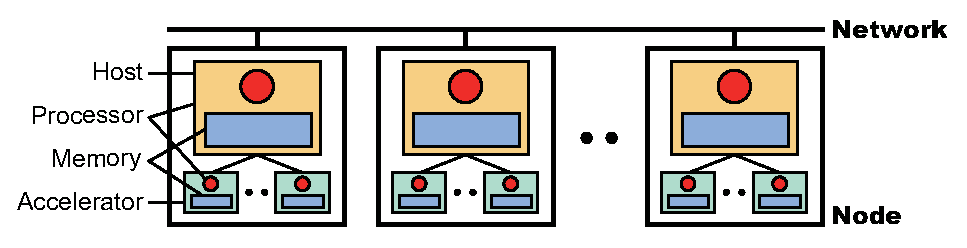
\includegraphics[width=\textwidth]{figs/hardware.eps}
  \caption{Hardware Model}\label{fig:hardware}
\end{myfigure}

An execution unit is called {\bf node} as with {\XMP}.
Each {\bf node} consists of a single host and multiple accelerators (such as GPUs and Intel MICs).
Each host has a processor, which may have several cores, and own local memory.
Each accelerator also has them.
Each {\bf node} is connected with each other via network.
Each {\bf node} can access its local memories directly and remote memories,
that is, the memories of another {\bf node} indirectly.
In a host,
the accelerator memory may be physically and/or virtually separate from the host memory as with the memory model of {\OACC}.
Thus,
a host may not be able to read or write the accelerator memory directly.

\subsection{Programming Model}
{\XACC} is a directive-based language extension based on Fortran 90 and ISO C90 (ANSI C90).
To develop applications on accelerated clusters with ease,
{\XACC} extends {\XMP} and {\OACC} independently as follow:
(1) {\XMP} extensions are to facilitate cooperation between {\XMP} and {\OACC} directives.
(2) {\OACC} extensions are to deal with multiple accelerators.

\subsubsection{{\XMP} Extensions}
In a program using the {\XMP} extensions,
{\XMP}, {\OACC}, and {\XACC} directives are used.
Fig. \ref{fig:concept} shows a concept of the {\XMP} extensions.

\begin{myfigure}
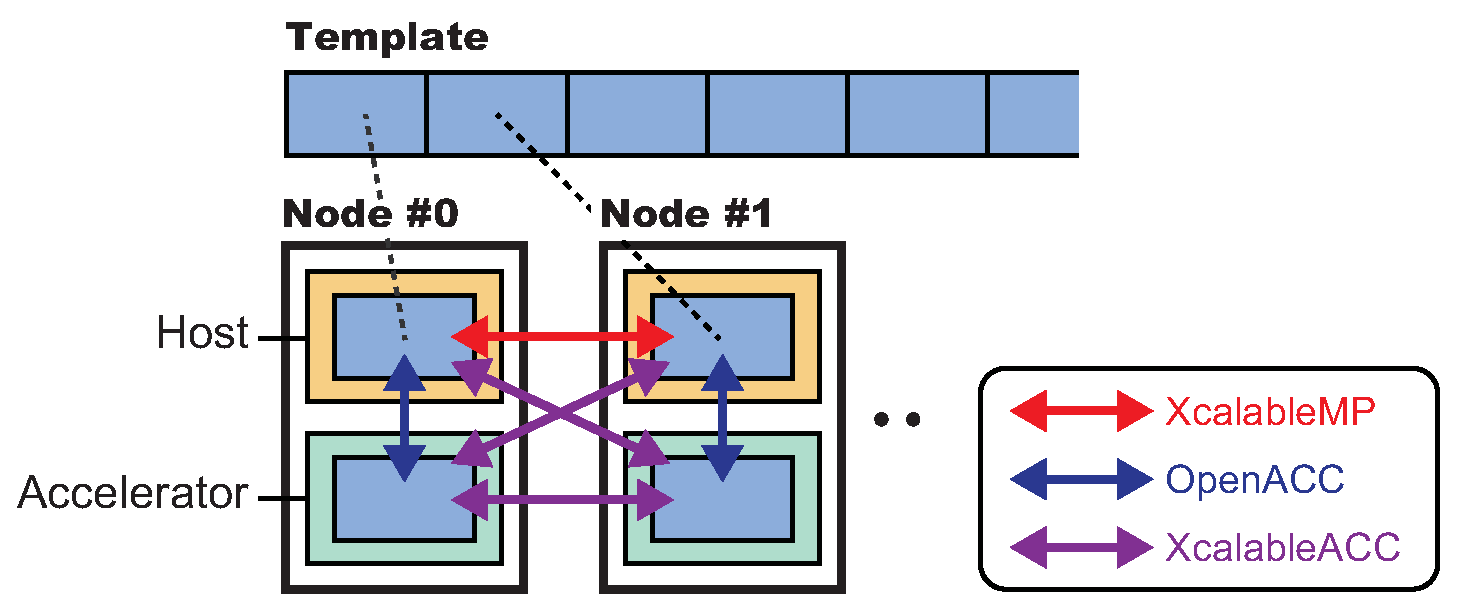
\includegraphics[width=\textwidth]{figs/concept.eps}
  \caption{Concept of {\XMP} Extensions}\label{fig:concept}
\end{myfigure}

{\XMP} directives define a {\bf template} and a {\bf node set}.
The {\bf template} represents a global index space, which is distributed onto the {\bf node set}.
Moreover, {\XMP} directives declare {\bf distributed arrays},
parallelize loop statements and transfer data among host memories according to the distributed {\bf template}.
{\OACC} directives transfer the {\bf distributed arrays} between host memory and accelerator memory on the same {\bf node}
and execute the loop statements parallelized by {\XMP} on accelerators in parallel.
{\XACC} directives, which are {\XMP} communication directives with an {\tt acc} clause, 
transfer data among accelerator memories and between accelerator memory and host memory on different {\bf nodes}.
Moreover, 
{\bf coarray} features also transfer data on different nodes.

%The {\XMP} extension is defined to develop parallel applications with keeping the sequential code image.
Note that 
the {\XMP} extensions are not a simple combination of {\XMP} and {\OACC}.
For example, 
if you represent communication of {\bf distributed array} among accelerators shown in Fig. \ref{fig:concept} by the combination of {\XMP} and {\OACC},
you need to specify explicitly communication between host and accelerator by {\OACC} and that between hosts by {\XMP}.
Moreover,
you need to calculate manually indices of the {\bf distributed array} owned by each {\bf node}.
By contrast,
{\XACC} directives can represent such communication among accelerators directly using global indices.

\subsubsection{{\OACC} Extensions}
The {\OACC} extension can represent offloading works and data to multiple-accelerators on a {\bf node}.
Fig. \ref{fig:concept_acc_ex} shows a concept of the {\OACC} extension.

\begin{myfigure}
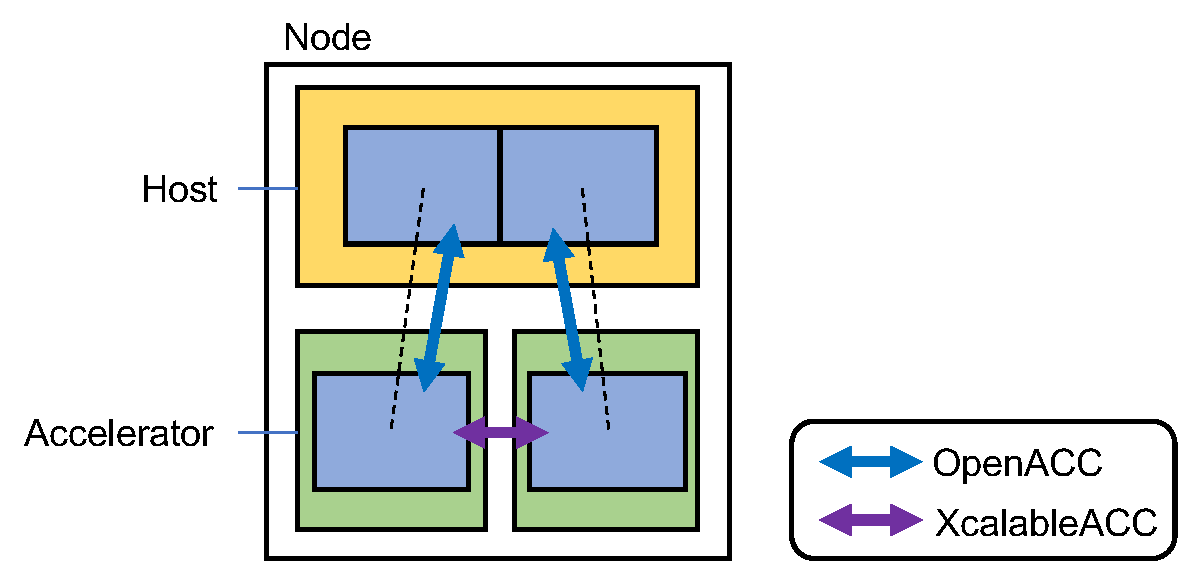
\includegraphics[width=\textwidth]{figs/concept_acc_ext.pdf}
  \caption{Concept of {\OACC} Extension}\label{fig:concept_acc_ex}
\end{myfigure}

{\OACC} extension directive defines a {\bf device set}.
The {\bf device set} represents a set of devices on a {\bf node}.
Futher, {\OACC} extension directives declare {\bf distributed arrays} on the {\bf device set} while maintaining the arrays on the host memory, and the directives distribute offloading loop statement and memory copy between host and device memories for the {\bf distributed-arrays}.
Moreover, {\OACC} extension directives synchronizes devices among the {\bf device set}.
{\XACC} directives also transfer data between device memories on the {\bf node}.

\subsection{Execution Model}
The execution model of {\XACC} is a combination of those of {\XMP} and {\OACC}.
While the execution model of a host CPU programming is based on that of {\XMP},
that of an accelerator programming is based on that of {\OACC}.
Unless otherwise specified,
each {\bf node} behaves exactly as specified in the {\XMP} specification\cite{xmp} or the {\OACC} specification\cite{openacc}.
%For details, refer to each specification\cite{xmp,openacc}.

An {\XACC} program execution is based on the SPMD model, 
where each {\bf node} starts execution from the same main routine and keeps executing the same code independently (i.e. asynchronously), 
which is referred to as the replicated execution
until it encounters an {\XMP} construct or an {\XMP}-extension construct.
In particular,
the {\XMP}-extension construct may allocate, deallocate, or transfer data on accelerators.
An {\OACC} construct or an {\OACC}-extension construct may define {\bf parallel regions}, such as work-sharing loops, 
and offloads it to accelerators under control of the host.

When a {\bf node} encounters a loop construct 
targeted by a combination of {\XMP} {\tt loop} and {\OACC} {\tt loop} directives,
it executes the loop construct in parallel with other {\bf accelerators},
so that each iteration of the loop construct is independently executed by the {\bf accelerator}
where a specified data element resides.

When a {\bf node} encounters a {\XACC} synchronization or a {\XACC} communication directive,
synchronization or communication occurs between it and other accelerators.
That is, such {\bf global constructs} are performed collectively by the {\bf current executing nodes}.
Note that neither synchronizations nor communications occur without these constructs specified.

\subsection{Data Model}
There are two classes of data in {\XACC}: {\bf global data} and {\bf local data} as with {\XMP}. 
Data declared in an {\XACC} program are local by default.
Both {\bf global data} and {\bf local data} can exist on host memory and accelerator memory.
About the data models of host memory and accelerator memory, refer to the OpenACC specification\cite{openacc}.

{\bf Global data} are ones that are distributed onto the {\bf executing node set} by the {\tt align} directive.
Each fragment of a {\bf global data} is allocated in host memory of a {\bf node} in the {\bf executing node set}.
{\OACC} directives can transfer the fragment from host memory to accelerator memory.

{\bf Local data} are all of the ones that are not global.
They are replicated in the local memory of each of the {\bf executing nodes}.

A {\bf node} can access directly only {\bf local data} and sections of {\bf global data} that are allocated in its local memory.
To access data in remote memory, 
explicit communication must be specified in such ways as the global communication constructs and the {\bf coarray} assignments.

Particularly in {\XACCF}, 
for common blocks that include any global variables, 
the ways how the storage sequence of them is defined and how the storage association of them is resolved are implementation-dependent.

% \subsection{Directive Format}
% This section describes the syntax and behavior of {\XMP} and {\OACC} directives in {\XACC}.
% In this document, 
% the following notation is used to describe the directives.

% \vspace{0.5cm}%
% \begin{tabular}{ll}
% {\tt xxx} & {\tt type-face} characters are used to indicate literal type characters. \\
% {\it xxx...} & If the line is followed by ``...'', then xxx can be repeated. \\
% {\it [xxx]} & {\it xxx} is optional. \\
% {\bsquare} & The syntax rule continues. \\
% \verb![F]! & The following lines are effective only in {\XACCF}. \\
% \verb![C]! & The following lines are effective only in {\XACCC}. \\
% \end{tabular}
% \vspace{0.5cm}%

% In {\XACCF}, 
% {\XMP} and {\OACC} directives are specified using special comments that are identified by unique sentinels {\tt\verb|!$xmp|} and {\tt\verb|!$acc|} respectively.
% the directives follow the rules for comment lines of either the Fortran free or fixed source form,
% depending on the source form of the surrounding program unit\footnote{Consequently, the rules of comment lines that an
% {\XMP} directive follows is the same as the ones that an {\OMP} directive follows.}.
% The directives are case-insensitive.

% \vspace{0.5cm}
% \Syntax{directive}
% \begin{tabular}{ll}
% \verb![F]! & \verb|!$xmp| {\it directive-name clause} \\
% \verb![F]! & \verb|!$acc| {\it directive-name clause} \\
% \end{tabular}
% \vspace{0.5cm}

% In {\XACC}, 
% {\XMP} and {\OACC} directives are specified using the \verb|#pragma| mechanism provided by the C standards.
% the directives are case-sensitive.

% \vspace{0.5cm}
% \Syntax{directive}
% \begin{tabular}{ll}
% \verb![C]! & \verb|#pragma xmp| {\it directive-name clause} \\
% \verb![C]! & \verb|#pragma acc| {\it directive-name clause} \\
% \end{tabular}
% \vspace{0.5cm}

%Directives are classified as {\bf declarative directives} and {\bf executable directives}\cite{xmp}.
%
%The {\bf declarative directives} are {\tt nodes}, {\tt template}, {\tt distribute}, {\tt align},
%{\tt shadow}, {\tt coarray}, {\tt declare}, and {\tt routine} directives.
%
%The {\bf executable directives} are {\tt template\_fix}, {\tt task}, {\tt tasks}, {\XMP} {\tt loop}, 
%{\tt array}, {\tt reflect}, {\tt reflect\_init}, {\tt reflect\_do}, {\tt gmove}, {\tt barrier}, 
%{\tt reduction}, {\tt bcast}, {\tt wait\_async},
%{\tt parallel}, {\tt kernels}, {\tt data}, {\tt host\_data}, {\OACC} {\tt loop},
%{\tt cache}, {\tt atomic}, {\tt init}, {\tt shutdown}, {\tt set}, {\tt update}, 
%{\tt wait}, {\tt enter\_data}, and {\tt exit\_data} directives.
%An {\bf executable directive} and its associated user code make up an {\XACC} construct, 
%as in the following format:
%
%\vspace{0.5cm}
%\begin{tabular}{ll}
%\verb![F]! & \verb|!$xmp| {\it directive-name clause} ...\\
% & \hspace{0.5cm} {\it structured-block} \\
%\verb![F]! & \verb|!$acc| {\it directive-name clause} ...\\
% & \hspace{0.5cm} {\it structured-block} \\
%\end{tabular}
%
%\vspace{0.3cm}
%
%\begin{tabular}{ll}
%\verb![C]! & \verb|#pragma xmp| {\it directive-name clause} ...\\
% & \hspace{0.5cm} {\it structured-block} \\
%\verb![C]! & \verb|#pragma acc| {\it directive-name clause} ...\\
% & \hspace{0.5cm} {\it structured-block} \\
%\end{tabular}
%\vspace{0.5cm}

% \subsection{Organization of This Document}
% The remainder of this document is structured as follows:

% \begin{itemize}
%  \item Chapter 2: {\XMP} Extensions
%  \item Chapter 3: {\OACC} Extensions
% \end{itemize}
 
%\cleardoublepage

\section{Coarray Features and the Key of the Implementation}\label{sec:lang}

XMP Fortran language specification supports a major part of coarray features defined in 
Fortran~2008 standard~\cite{F08}, and intrinsic procedures 
{\tt CO\_SUM}, {\tt CO\_MAX}, {\tt CO\_MIN} and {\tt CO\_BROADCAST} defined in 
Fortran~2018 standard~\cite{F18} were supported.
And also XMP C language specification extended to support coarray features.

This section introduces the coarray features and what is required
to the compiler in order to implement the coarray features.


%-----------------------------------------------------------------------------
\subsection{Images Mapped to XMP Nodes}
%-----------------------------------------------------------------------------

In the Fortran standard, an {\bf image} is defined as a instance of a program. 
Each image executes the same program and has its own data individually 
(SPMD: Single Program/Multiple Data).
Each image has a different image index, which is one of $1, \cdots, n$, 
where $n$ is the number of images. 
While Fortran standard does not specify actually where each image is executed, 
XMP defines that the images are mapped in tern to the executing nodes. 
Therefore, image $k$ is always executed simply on executing node $k$, 
where $1 \leq k \leq n$ and 
$n$ is the number of images and also the number of the executing nodes. 

Note that the executing nodes can be a subset of the entire (initial) node set. 
For example, two distinct node sets can execute two coarray subprograms concurrently.
When the execution encounters a {\tt TASK} directive specified with a subset of nodes,
the corresponding subset of the images will be the executing images for the
TASK region. 
The number of images and my image number, which are given by inquire functions
{\tt num\_images} and {\tt this\_image}, also match with the executing images, and
the {\tt SYNC\_IMAGES} statement synchronizes among the executing images.
When the execution encounters the {\tt END TASK} directive corresponding to the
{\tt TASK} directive, the set of executing image is reinstated.
Unless the {\tt TASK} and {\tt END TASK} directives are used, coarray features are 
compatible to the ones of the Fortran standard. 

%   Coarray features can be used inside the TASK directive blocks. As default,
%   each coarray image is mapped one-to-one to a node of the current executing 
%   task. I.e., num_images() returns the number of nodes of the current executing 
%   task and this_image() returns each image index in the task.
%      There are two directives to change the default rule above. A COARRAY 
%   directive corresponding to a coarray declaration changes the image index set 
%   of the specified coarray with the one of the specified nodes. An IMAGE 
%   directive corresponding to one of a SYNC ALL statement, a SYNC IMAGES 
%   statement, a call statement calling CO_SUM, CO_MAX, CO_MIN or CO_BROADCAST 
%   changes the current image index set with the one of the specified nodes.
%   See the language spacifications [3].


\requirement
Memory management is necessary to cope with changes of the executing images.

%The XMP compiler manages these values in stack.
%タスク実行のときのスタックの使い方、構文が入れ子なので同じレベルに戻ることができること。


%-----------------------------------------------------------------------------
\subsection{Allocation of Coarrays}
%-----------------------------------------------------------------------------

A {\bf coarray} or a coarray variable is a variable that can be referred from the other images. 
A coarray with the {\tt ALLOCATABLE} attribute is called an {\bf allocatable coarray}, 
otherwise called a non-allocatable coarray. A non-allocatable coarray may not be a pointer 
and must have an explicit shape and the {\tt SAVE} attribute. 
In order to help intuitive understanding, we call a non-allocatable coarray as 
a {\bf static coarray}. The lifetime of a static coarray is throughout execution of the program. 
On the other hand, an allocatable coarray is allocated with the {\tt ALLOCATE} statement and 
freed either explicitly with the {\tt DEALLOCATE} statement or implicitly at the end of the scope
in which the {\tt ALLOCATE} statement is executed ({\bf automatic deallocation}).

Static coarrays can be declared as scalar or array variables as follows:
\begin{verbatim}
      real(8), save :: a(100,100)[*]
      type(user_defined_type), save :: s[2,2,*]
\end{verbatim}

The square bracket notation in the declaration distinguishes coarray variables from 
the others (non-coarrays). It declares the virtual shape of the images and the last 
dimension must be deferred (as `{\tt *}').

Allocatable coarrays can be declared as follows:
\begin{verbatim}
      real(8), allocatable :: b(:,:)[:]
      type(user_defined_type), allocatable :: t[:,:,:]
\end{verbatim}


A notable constraint is that at any synchronization point in program execution, 
coarrays must have the same dimensions (sizes of all axes) between all images
({\bf symmetric memory allocation}). 
Therefore, an static coarray must have the same shape between all images during 
the program execution, and an allocatable coarray must be allocated and deallocated 
collectively at the same time with the same dimensions between the executing images.
Thanks to the syn-metric memory allocation rule, all executing images can have
the same symmetrical memory layout, which makes it possible to calculate the address 
of the remote coarray with no prior inter-image communication.

% 2. Declaration
%   Either static or allocatable coarray data objects can be used in the program. 
%   Use- and host-associations are available but common- or equivalence-
%   association are not allowed in conformity with the Fortran2008 standard.
%   Current restrictions against Fortran2008 coarray features:
%     * Rank (number of dimensions) of an array may not be more than 7.
%     * A coarray cannot be of a derived type nor be a structure component.
%     * A coarray cannot be of quadruple precision, i.e., 16-byte real or 32-byte 
%       complex.
%     * Interface block cannot contains any specification of coarrays. To describe
%       explicit interface, host-assocication (with internal procedure) and use-
%       association (with module) can be used instead.
%     * A pointer component of a derived-type coarray is not allowed.
%     * An allocatable component of a derived-type coarray cannnot be referrenced
%       as a coindexed object.
%     * A derived-type coarray cannot be defined as allocatable.

% 2.1  Static Coarray
%   E.g.
%       real(8) :: a(100,100)[*], s(1000)[2,2,*]
%       integer, save :: n[*], m(3)[4,*]
%   The data object is allocated previously before the execution of the user 
%   program.  A recursive procedure cannot have a non-allocatable coarray without 
%   SAVE attribute.
%   Current restrictions against Fortran2008 coarray features:
%     * Each lower/upper bound of the shape must be such a simple expression that 
%       is an integer constant literal, a simple integer constant expression, or
%       a reference of an integer named constant defined with a simple integer 
%       constant expression.
%     * A coarray cannot be initialized with initialization or with a DATA 
%       statement.
%     
% 2.2  Allocatable Coarray
%   E.g.
%       real(8), allocatable :: a(:,:)[:], s(:)[:]
%       integer, allocatable, save :: n[:], m(:)[:,:]
%   The data object is allocated with an ALLOCATE statement as follows:
%       allocate ( a(100,100)[*], s(1000)[2,2,*] )
%   The allocated coarray is deallocated with an explicit DEALLOCATE statement or 
%   with an automatic deallocation at the end of the scope of the name unless it 
%   has SAVE attribute.
%   Current restrictions against fortran2008 coarray features:
%     * A scalar coarray cannot be allocatable.
%     * An allocatable coarray as a dummy argument cannot be allocated or 
%       deallocated inside the procedure.

\requirement
The language specification suggests the compiler to maintain the symmetric memory
allocation rule and to use it for efficient remote address calculation.

automatic deallocationの生成が必要なことをどこかに書いたか?

%-----------------------------------------------------------------------------
\subsection{Communications}
%-----------------------------------------------------------------------------

Coarray features include three types of communications between images, i.e.,
\begin{itemize}
\item reference and definition to remote coarrays (GET and PUT communication),
\item collective communication (intrinsic subroutines {\tt CO\_SUM}, {\tt CO\_MAX}, 
{\tt CO\_MIN} and {\tt CO\_BROADCAST}), and
\item atomic operations ({\tt ATOMIC\_DEFINE} and {\tt ATOMIC\_REF}).
\end{itemize}

Omni compiler implements the latter two communications using the corresponding 
functions in MPI. The rest of this section describes the former communication.

%===========================================================
\subsubsection{PUT communication}\label{sec:PUT}
%===========================================================

PUT communication is caused by an assignment statement with a {\bf coindexed variable} 
as the left-hand side expression, e.g.,
\begin{verbatim}
      a(i,j)[k] = alpha * b(i,j) + c(i,j)
\end{verbatim}
This statement is to cause the PUT communication to the array element $a(i,j)$ on image $k$
with the value of the left-hand side.

Fortranの配列代入文を使えば、配列から配列へのPUT通信を記述することもできる。
例えば以下の配列代入文は、$M N$ 要素のPUT通信を生じさせる。
\begin{verbatim}
      a(1:M,1:N)[k] = alpha * b(1:M,1:N) + c(1:M,1:N)
\end{verbatim}

\requirement
配列代入文では、一般には右辺の評価結果をFortranシステムが一時領域に置くが、
通信バッファをできる限り多重にしない工夫が必要である。
右辺が配列の参照だけの場合はゼロコピー通信とすることが望ましい。
また、次のimage制御文によって同期が行われるまでPUTされたデータは他のimageから
参照されないので、実行はPUT通信の完了を待たないで次に進むことができる(non-blocking communication)。


%===========================================================
\subsubsection{GET communication}\label{sec:GET}
%===========================================================

GET communication is caused by referencing the {\bf coindexed object}, 
which is represented by a coarray variable with cosubscripts enclosed by square brackets, 
e.g., $s[1,2]$ and $a(i,j)[k]$, where $s$ and $a$ are scalar and two-dimensional array coarrays,
respectively.
Coindexed objects can appear in most expressions.

値を配列とする配列式を使うと配列に対するGET通信を行うことができる。
例えば coindexed-object $a(1:M,1:N)[k]$ の値は$a$と同じ型で形状$[M, N]$の2次元配列である。


\requirement
ローカル側は、獲得したデータがすぐに消費されることからnon-blocking化は適さない。
できる限りバッファリングを回避してゼロコピーとすることで効率化したい。
受信側(local側)をゼロコピーにするため、最適化が有効。右辺に1つのcoindexed-object1しかない
配列代入文、例えば、
\begin{verbatim}
      a(1:M,1:N) = b(1:M,1:N)[k]
\end{verbatim}
では、GET通信の受信先をバッファでなく直接変数aにすることで、ゼロコピーにできる場合がある。


%-----------------------------------------------------------------------------
\subsection{Inter-image Synchronization}
%-----------------------------------------------------------------------------
Basically, the Fortran language specification does not guarantee the inter-image 
data dependency unless any image control statements are explicitly used.
\fig{sync-ex} shows an example of program fragment describing inter-image communication
and synchronization by the reference and definition of coarrays and {\tt SYNC ALL} statement.
Here, all variables {\tt a}, {\tt b}, {\tt c}, {\tt x}, {\tt y} and {\tt z} are coarrays.
%
An {\bf image control statement}, such as {\tt SYNC ALL} and {\tt SYNC IMAGES} statements, 
separates a procedure into {\bf segments}. In \fig{sync-ex}, portions between lines~2 and 9 and 
between lines~11 and 20 are segments.
The synchronization between images does not need to complete until encountering the 
image control statements. And the compiler optimization does not allowed to perform 
the code motion across the image control statement. In \fig{sync-ex}, 
{\tt sync all} in line~10 should wait for completion of the definition to coarray {\tt a} 
in line~4, and should prevent the code motion of lines~4 and 5 and lines~16, 17 and 19 
from crossing the {\tt sync all} in line~10.

緩い同期である。ここに最適化のチャンスがある。

\begin{figure}[hbt]
 \begin{center}
\begin{verbatim}
 1      sync all
 2
 3      if (this_image()==1) then
 4          a[2]=
 5          b[2]=
 6          =c[2]
 7          x=
 8          y=
 9          =z
10      endif
11
12      sync all
13
14      if (this_image()==2) then
15          =a
16          b=
17          c=
18          =x[1]
19          y[1]=
20          z[1]=
21      endif
22
23      sync all

\end{verbatim}
  \caption{Example of inter-image synchronization}
  \label{fig:sync-ex}
 \end{center}
\end{figure}



各イメージの中では、従来のFortran仕様に従う依存関係の維持が必要である。
non-coarrayデータに関しては従来とおりだが、coarrayについて注意が必要。
In order to keep data dependency among the definitions and 
references in the coarray, the non-blocking communication should be restricted.
\fig{block-ex} にdata dependencyに気をつけなければならない例を示す。
同じリモートデータに対して同じsegment内で複数回アクセスする場合である。

\begin{figure}[hbt]
 \begin{center}
\begin{verbatim}
 1      if (this_image()==2) then
 2          a[2]=
 3          =a[2]     ! should wait for the completion of line 2 to keep flow dependency.
 4          a[2]=     ! should wait for the completion of line 3 to keep anti dependency.
 5      endif

\end{verbatim}
  \caption{Example of intra-image communication blocking}
  \label{fig:block-ex}
 \end{center}
\end{figure}


\requirement
To reduce the latency overhead, non-blocking one-sided communication is effective.
The compiler should generate non-blocking GET communication as long as possible.
In usual case, the completion point of the non-blocking is the end of the segment, as
shown in \fig{sync-ex}.  However, the possibility to meet the condition shown in
\fig{block-ex} should be took account. If the PUT communication is always in blocking, 
only the flow dependency should be care; the previous PUT communication (line~2) 
should be completed before the following GET communication (line~3).

%-----------------------------------------------------------------------------
\subsection{Subarrays and Data Contiguity}
%-----------------------------------------------------------------------------

In Fortran, if an array, except dummy argument, is declared as {\tt real a(1:M,1:N)}, 
the reference to the whole array (i.e., {\tt a} or {\tt a(:,:)} or {a(1:M,1:N)})
is defined {\bf contiguous}. 
We defined a term {\bf contiguous length} as the length how long the data is partially
contiguous. For example, the contiguous lengths of {\tt a(2,3)} and {\tt a(2:5,3)} are
1 and 4 respectively.  {\tt a(1:M,1:3)} is two-dimensionally contiguous and has 
contiguous length $2 \times {\tt M}$.
{\tt a(1:M-1,1:3)} is one-dimensionally contiguous and has 
contiguous length $({\tt M} - 1)$.


\requirement
通信の高速化のためには,十分に長い範囲の連続性を実行時に抽出する必要がある.
一般にノード間通信で立ち上がりレイテンシ時間がほぼ無視できるようになるデータ量は
数千バイトであることから,配列や部分配列の1次元め(Fortranでは1番左の添字)が
連続であっても数千要素に満たない場合には,次元を跨いだ連続性まで抽出して,
十分に長い連続データとして通信する技術が必要である.
【fx100-latencyのグラフから数千バイトを言ってもよい。】

GET通信と同様,a(i,j)[k]は代わりに全体配列にも部分配列にもなれるので,
coindexed variableについても次元を跨いだ連続性の抽出が必要である.
それに加えて、ローカル側、すなわち、右辺式データの連続性も意識に入れなければならない。
高速な通信を実現するには,左辺と右辺で共通に連続な区間を検出してその単位で通信を反復するか,
右辺データは連続区間にpackして左辺の連続区間を単位として通信を反復するなどの戦略がある。



%-----------------------------------------------------------------------------
\subsection{Coarray C Language Specifications}
%-----------------------------------------------------------------------------

C言語にも配列式、配列代入を導入することでFortranと同様なcoarray featuresを仕様定義した。

coarrayはデータ実体に限る。ポインタはcoarrayになれない。形式的には、
1)基本型、2)ポインタを含まない構造型、または、3) 1or2or3の配列とする。
Cのcoarrayにおいてもstaticとallocatableがある。ファイル直下で宣言するか
static指示したcoarrayはstatic coarrayである。ライブラリ関数xxxをつかって
割付けたデータ領域はallocatable coarrayであり、ライブラリ関数は
allocatable coarrayへのポインタを返す。
Cのcoarrayは、通常のCの変数と同じように、引数渡しやcast演算によって自由に
その型と形状の解釈を変えることができる。

これらの仕様と制限は、Cプログラマ
にとっての使いやすさを考えて、Cらしいプログラミングスタイルを認めた。
Coarray C++とは違うアプローチである。

cf.\ air:/Users/iwashita/Desktop/coarray/Project\_Coarray/の下にいくつか

%\cleardoublepage

\section{Implementation}\label{sec:implement}

%-----------------------------------------------------------------------------
\subsection{Omni XMP Compiler Framework}
%-----------------------------------------------------------------------------

The CAF translator was added to the Omni XMP compiler~\cite{omni}, 
as shown in Figure~\ref{fig:translator}.
The Omni XMP compiler is a source-to-source translator that converts XMP programs 
into the base language (Fortran or C). The component 'coarray translator' is 
located in front of the XMP translator to solve coarray features previously.   
The output of the decompiler is a standard Fortran/C program, which may include 
calls to the XMP runtime library.

The following procedures are generated in advance or in the coarray translator
to initialize static coarray variables prior to the execution of the user program:
\begin{itemize}
\item
The built-in main program calls subroutine {\tt xmpf\_traverse\_init},
the entry procedure of initialization subroutines, before executing the
user main program.
\item
Subroutine {\tt xmpf\_traverse\_init} is generated by the coarray translator 
to call initialization subroutines corresponding to all user-defined procedures.
\item
Each initialization subroutine {\tt xmpf\_init\_{\it foo}} is generated from 
user-defined procedure {\it foo} by the coarray translator, which initializes all static coarrays declared in {\it foo}.
\end{itemize}

\begin{figure}[tbh]
 \begin{center}
  % trimはleft bottom right topの順
  %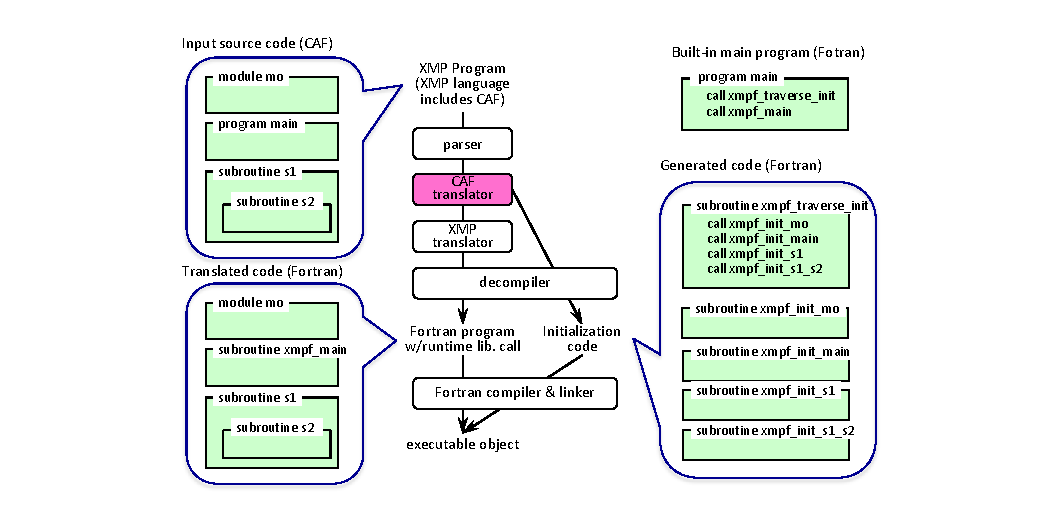
\includegraphics[scale=0.55,trim=6cm 0cm 4cm 6cm,clip]{figs/translator-tmp.pdf}
  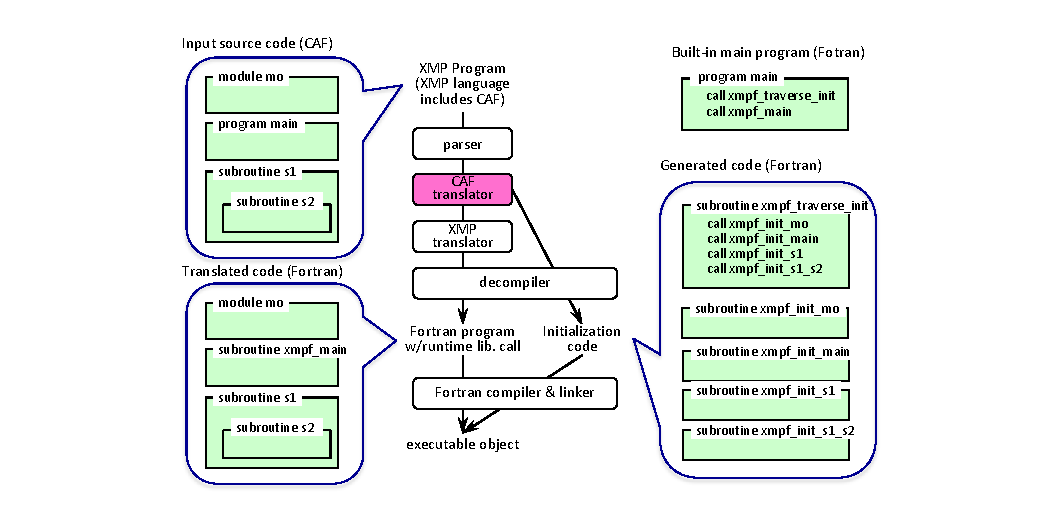
\includegraphics[trim=30mm 0mm 20mm 7mm, scale=1.0]{figs/translator-tmp.pdf}
  \caption{XMP compiler and an example of coarray program compilation}
  \label{fig:translator}
  %-- 修正すべき箇所
  CAF translator $\rightarrow$ coarray translator
 \end{center}
\end{figure}


%-----------------------------------------------------------------------------
\subsection{Allocation and Registration}\label{sec:alloc}
%-----------------------------------------------------------------------------

In order to be accessed using the underlying communication library,
the allocated coarray data must be registered to the library.
The registration contains all actions to allow the data to be accessed 
from the other nodes, including pin-down memory, acquirement of the global address,
and sharing information among all nodes.

%===========================================================
\subsubsection{Three Methods of Memory Management}
%===========================================================

The coarray translator and the runtime library implements three methods of
memory management.
\begin{itemize}
\item
The {\bf runtime sharing (RS) method} allocates and registers a large memory 
for all static and dynamic coarrays at the initialization phase.
The registered memory is shared by all static and allocatable coarrays. 

\item
The {\bf runtime allocation (RA) method} allocates and registers a large memory
for all static coarrays at the initialization phase.
The RA method also allocates and registers each allocatable coarray at runtime.

\item
The {\bf compiler allocation (CA) method} allocates all coarray objects by 
the Fortran system (at compile time or at runtime), and the address is 
passed to the runtime library to be registered.
\end{itemize}

For the RS and RA methods, 
since the allocated memory address is determined in the runtime library, 
the object code must accept the address allocated 
inside the runtime system as an address of a regal Fortran variable.
To make this connection, it was necessary to use the Cray pointer, which is not 
in the Fortran standard.
In the case of the CA method, the runtime library accepts the address allocated
in the Fortran system and registers to the communication library.

%
% 3 methodsの比較表を載せるならここか
%


%===========================================================
\subsubsection{Initial Allocation for Static Coarrays}
%===========================================================

Static coarrays are allocated and registered in the initialization subroutines 
{\tt xmpf\_init\_{\it foo}}. 

Using the RS and RA methods, static coarrays are initialized before execution of the user program,
as follows.
\begin{itemize}
\item
In the first pass, all sizes of static (non-allocatable) coarrays are summed.
The size of each static coarray is evaluated form the lower and upper bounds
specified in the dimension declaration statement of each coarray.
The lower and upper bound expressions, possibly including binary and unary
operations, references to names of constants, and basic intrinsic functions, 
such as min/max and sum, are evaluated by constant folding.
Since the size of the structure that contains allocatable or pointer 
components differs depending on the target compiler, the coarray translator
obtains the necessary parameters to calculate the size of structures at build time.
\item
Then, the total size of static coarrays is allocated and the address
and size are registered to the underlying communication library.
\item
In the second pass, the addresses of all of the coarrays are calculated to share
the registered data.
Due to the language specification, the sizes of the same coarray are the same 
among all images (nodes). Therefore, the offset from the base address of the registered 
data for each coarray can be the same among all images.
\end{itemize}
%
In the RS method, allocatable coarrays also share the registered memory. 
The total size of the memory to be registered
should be specified with an environment variable by the user.
In the RA method, the total size is fully calculated by the runtime 
library, and no information is required of the user because allocatable coarrays
will be dynamically allocated on the other memories.

In the CA method,
the Fortran processor allocates each coarray, and the runtime library
then registers the address.
Each static coarray is converted into a common (external) variable to share 
between the user-defined procedure (say {\it foo}) and its initialization
procedure ({\tt xmpf\_init\_{\it foo}}). The data is statically allocated
by the Fortran system in a manner similar to the usual common variable.
The address is registered in the initialization procedure via the runtime library.

%===========================================================
\subsubsection{Runtime Allocation for Allocatable Coarrays}
%===========================================================

For the RS method, the runtime library has a memory management system for
cutting out and retrieving memory for each allocation and deallocation of coarrays.

Figure~\ref{fig:register-RA-CA} illustrates the memory allocation and registration
for allocatable coarrays in the RA and CA methods. 

\begin{figure}
 \begin{center}
  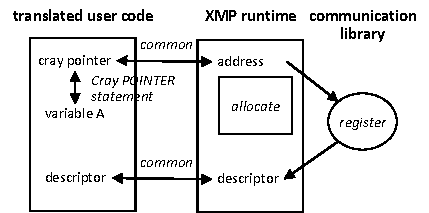
\includegraphics[scale=0.9, trim=0mm 0mm 0mm 0mm, clip]{figs/register-RA-tmp.pdf}\\
The runtime allocates and registers coarrays and passes the address to the user code.
 \end{center}
 \begin{center}
(a) RA method
 \end{center}
 \begin{center}
  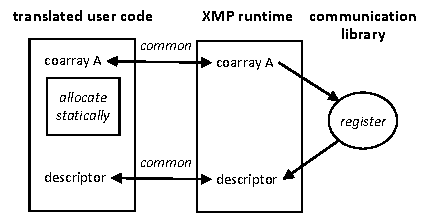
\includegraphics[scale=0.9, trim=0mm 0mm 0mm 0mm, clip]{figs/register-CA-tmp.pdf}\\
The user code allocates coarrays and causes the runtime to register with the address.
 \end{center}
 \begin{center}
(b) CA method
 \end{center}
 \caption{Memory allocation for coarrays in RA and CA methods}
 \label{fig:register-RA-CA}
\end{figure}

These methods are properly used by the underlying communication library.
%
For GASNet, only the RS method is adopted because its allocation function
can be used only once in the program.
%
For MPI-3, the CA method is not suitable because frequent 
allocation and deallocation of coarrays cause expensive creation and freeing of 
MPI windows.
%
In the case of FJ-RDMA, the RS method has no advantage over the other methods.
Since the allocated address is used for registration to FJ-RDMA, 
no advantage was found for managing memory outside of the Fortran system. 
The unusual connection through the Cray pointer causes degradation of 
the Fortran compiler optimization.


%-----------------------------------------------------------------------------
\subsection{PUT/GET Communication}\label{sec:putget}
%-----------------------------------------------------------------------------

In order to avoid disturbing the execution on the remote image, PUT and GET communications
are always implemented using remote direct memory access (RDMA) provided by 
the communication library (except coarrays with pointer/allocatable structure components). 
In contrast, local data access is selective between using direct memory access (DMA) or
using a local buffer. For the buffer scheme, one of four algorithms will be chosen.


%===========================================================
\subsubsection{Determining the Possibility of DMA}\label{sec:opt-dma}
%===========================================================

Coarray variables must be registered when allocated to be 
the target of RDMA communication. In contrast, since the local
data, which is the source of PUT or the destination of GET,
was not registered or linked to registered information,
the data could not be the target of DMA communication and had to be communicated via the registered buffer.

When the local data is an entire coarray or a part of coarray,
the coarray must be registered, and efficient DMA-RDMA communication can 
be made. Since the analysis at compile time is limited,
we implemented the detector in the runtime library 
using binary-tree search, as follows.
%
\begin{enumerate}
\item
When a chunk of coarray data is registered to the communication library, 
the runtime library adds the set of the local address and the size to a sorted 
table called {\tt SortedChunkTable}. The sort key is the local base address
of the data.
\item
When a chunk of coarray data is deregistered from the communication library, the 
runtime library deletes the record in {\tt SortedChunkTable}.
\item
When a PUT or GET runtime library is called corresponding to a reference/definition
to a coindexed object/variable, the local address is searched in {\tt SortedChunkTable}
with binary search. The local data is already registered if 
$addr_i \leq addr < addr_i + size_i$ for any $i$,
where $addr$ is the said local address and $add_i$ and $size_i$ are the
$i$-th address and size, respectively, in {\tt SortedChunkTable}.
\end{enumerate}

If the communication data is large, then the cost of procedure 3 is relatively small
and is worth using. 
If the data is small, then the buffering algorithm, as shown in \Sec{buffer}, may be better.


%===========================================================
\subsubsection{Buffering Communication Methods}\label{sec:buffer}
%===========================================================

For the buffer scheme, one of four algorithms will be chosen 
depending on three parameters: the size of the local buffer $B$ and the 
local and remote contiguous lengths $N_L$ and $N_R$, respectively.
Here, $B$ should be large enough to ignore communication latency overhead and we use
approximately 400 kilo-bytes by default. Unlike the case of MPI message passing,
coarray PUT/GET communication requires only one local buffer for any number of
other images.
Both $N_L$ and $N_R$ can be evaluated at runtime. The Fortran syntax guarantees 
that $N_L$ is a multiple of $N_R$ or $N_R$ is a multiple of $N_L$.
An algorithm to obtain the contiguous length is shown in a previous paper~\cite{pgas15}.

\tab{putget} summarizes our algorithm for PUT/GET communication for five cases.
The unit size is the chunk length of the PUT/GET communication.
Case~0 shows the algorithm using RDMA-DMA PUT/GET communication, and Cases~1 through~4 show the algorithms using RDMA and local-buffering. 
Due to its strict condition, the DMA scheme is rarely used.
In addition, this scheme is not always faster than the buffering scheme for Cases~2 and~3 because of the difference in the unit sizes. The advantage of Cases~2 and~3 is that the unit size 
is extended to a multiple of $N_L$ by gathering a number of short contiguous data in the buffer,
or by scattering from the buffer into a number of short contiguous data.

\begin{table}[tbh]
 \caption{Summary of the PUT/GET algorithm related to $N_L$, $N_R$, and $B$}
 \label{tab:putget}
 \begin{flushleft}
  \begin{tabular}{|@{~}c@{~}|c||@{~}c@{~}|@{~}c@{~}|}
\hline
Scheme &
Case &
Condition &
Unit size \\
\hline
\hline
DMA &
&
local data is registered &
$\min(N_L, N_R)$ \\
\hline
Buffering &
1 & 
$N_R \leq B,~ N_R \leq N_L$ &
$N_R$ \\
\cline{2-4}
&
2 &
$N_L < N_R \leq B$ &
$N_R$ \\
\cline{2-4}
&
3 &
$N_L < B < N_R$ &
multiple of $N_L$ ($\leq B$) \\
\cline{2-4}
&
4 &
$B < N_R,~ B \leq N_L$ &
$B$ (or less than $B$ at last) \\
\hline
  \end{tabular}
 \end{flushleft}
 \begin{flushleft}
  \begin{tabular}{|@{~}c@{~}|c||@{~~}l@{~~}|@{~~}l@{~~}|}
\hline
Scheme &
Case &
PUT action for each unit &
GET action for each unit \\
\hline
\hline
DMA &
&
put once &
get once \\
\hline
Buffering &
1 &
buffer once, and put once &
get once, and unbuffer once \\
\cline{2-4}
&
2 &
buffer for each $N_L$, and put once &
get once, and unbuffer for each $N_L$ \\
\cline{2-4}
&
3 &
buffer for each $N_L$, and put once &
get once, and unbuffer for each $N_L$ \\
\cline{2-4}
&
4 &
buffer once, and put once &
get once, and unbuffer once \\
\hline
  \end{tabular}
 \end{flushleft}
\end{table}


%===========================================================
\subsubsection{Non-blocking PUT Communication}
%===========================================================

For higher performance, the PUT communication should be non-blocking, and
the completion wait should be delayed until the end of the segment.
Writing and reading the same remote data from
the same image in the same segment appears to be a very rare case, as described in \Sec{spec-sync}.
However, this is difficult to detect with low cost. Since the subscripts and image
indices are often variable expressions, the compiler rarely select non-blocking communication
and usually generates safe but slow code.
We do not have a reasonable solution for this issue.

In the current implementation, the user selects blocking or non-blocking for
PUT communication at runtime with the environment variable.
%ほとんどの場合には該当しないことを利用者が分かるので、non-blockingのオプションを
%選択することを期待する。


%===========================================================
\subsubsection{Optimization of GET Communication}\label{sec:opt-get}
%===========================================================

A reference to an array-coindexed object is converted to a call of a runtime library 
function that returns a Fortran array value. For example, array assignment statement:
\begin{verbatim}
 b(j1:j2) = a(i1:i2)[k] 
\end{verbatim}
is converted to
\begin{verbatim}
 b(j1:j2) = xmpf_coarray_get_generic(dp_a,k,a(i1:i2)) 
\end{verbatim}
by the coarray translator, where {\tt dp\_a} is the descriptor of coarray {\tt a}.
The issue is that the result of the library function is an array value, which
causes several memory copies.
% The result value of the function is one-dimensional array whose size 
% is $({\tt i2} - {\tt i1} + 1)$.
% The issue is that it tends to cause many data copies in some library layers.
As a countermeasure, we optimized a specific but common case by the translator.
If a coindexed object is only the right-hand side of an array assignment statement, then
the entire assignment statement can be converted into a single library call.
The above example satisfies this condition and so can be converted again as follows:
\begin{verbatim}
 call xmpf_coarray_getsub_generic(dp_a,k,a(i1:i2),b(j1:j2)) 
\end{verbatim}
In this runtime library subroutine, the variable {\tt b(j1:j2)} is expected to be 
the local target of GET communication, instead of the local buffer that would be
generated by the Fortran runtime.


%-----------------------------------------------------------------------------
\subsection{Runtime Libraries}\label{sec:runtime}
%-----------------------------------------------------------------------------

The layer of the runtime libraries is shown in \fig{layer}.
One of three communication libraries is selected 
at the build time of the Omni compiler.
The coarray runtime consists of three layered libraries.
%
The {\bf Fortran wrapper} mediates the arguments and the result value 
of the translated user program (written in Fortran) and the upper-layer runtime (ULR) (written in C).
%
The {\bf (ULR) library} performs the algorithms 
described above in this section.
%
The {\bf lower-layer runtime (LLR) library} abstracts the difference between 
the communication libraries, except for the memory management of coarray data.

\begin{figure}[tbh]
  \begin{center}
    % trimはleft bottom right topの順
    %\mbox{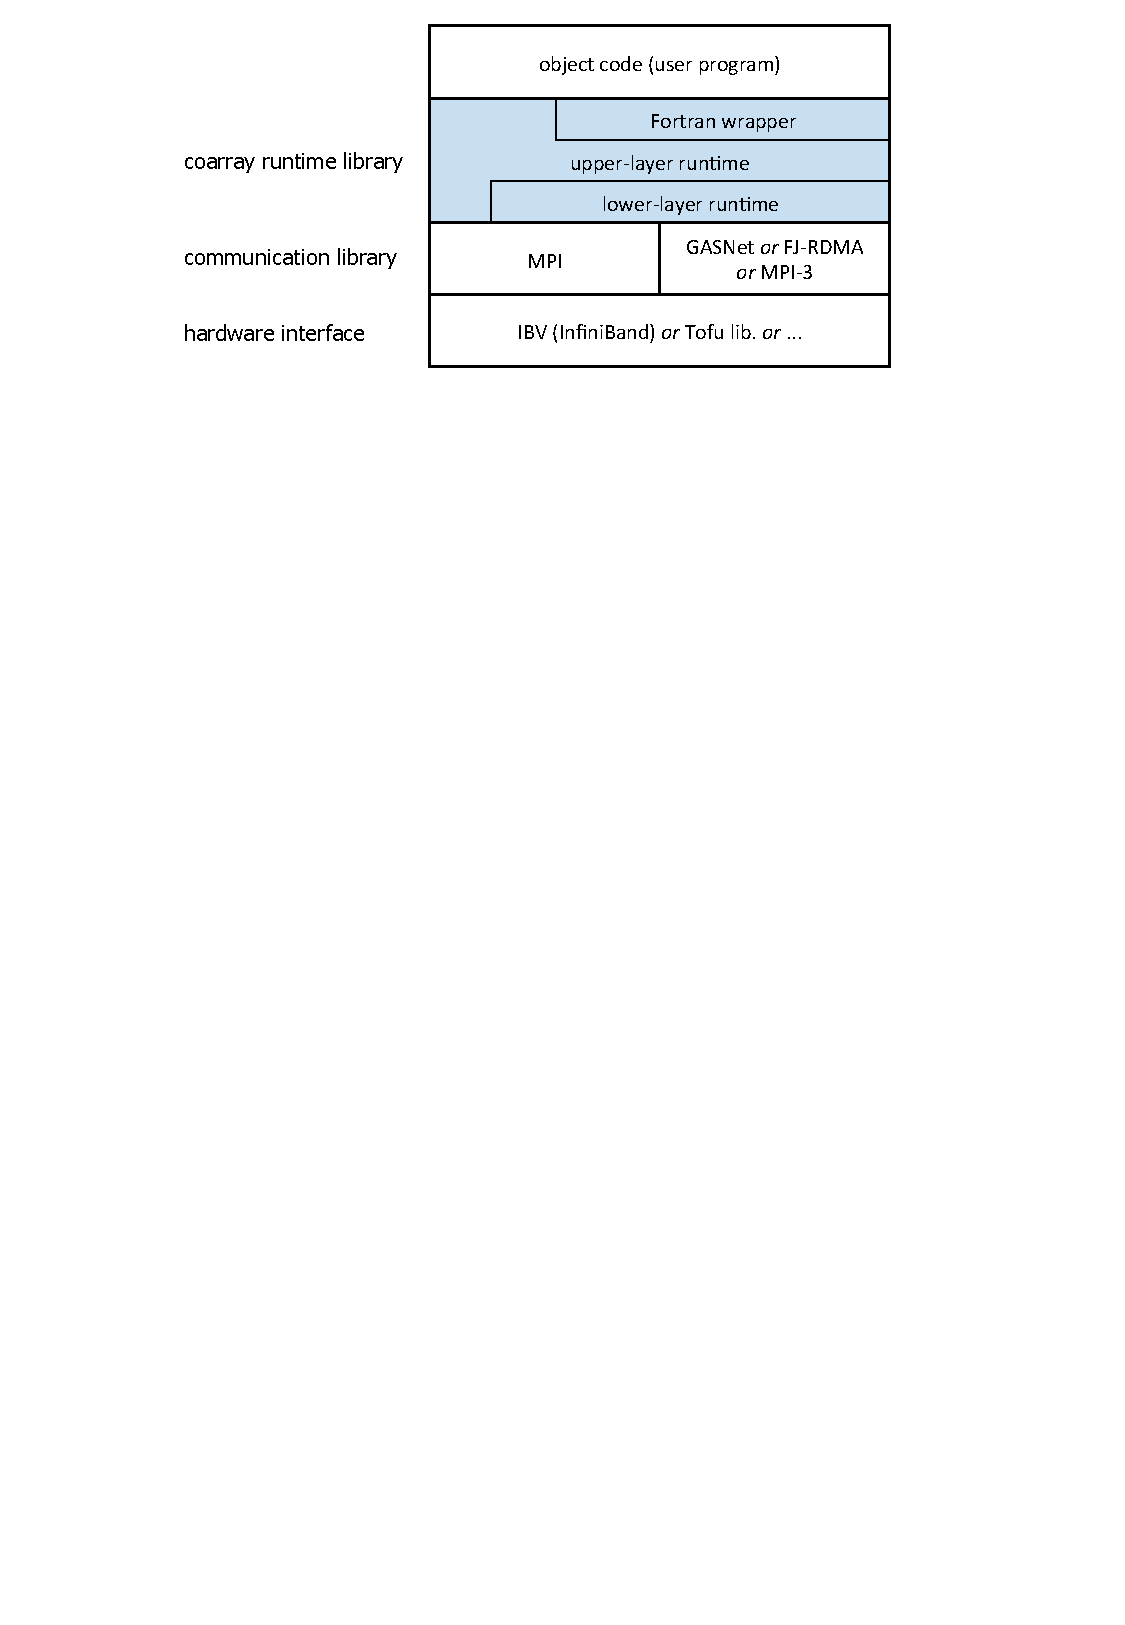
\includegraphics[trim=42mm 210mm 47mm 0mm, scale=0.7,clip]{figs/softstack-r2.pdf}}
    \mbox{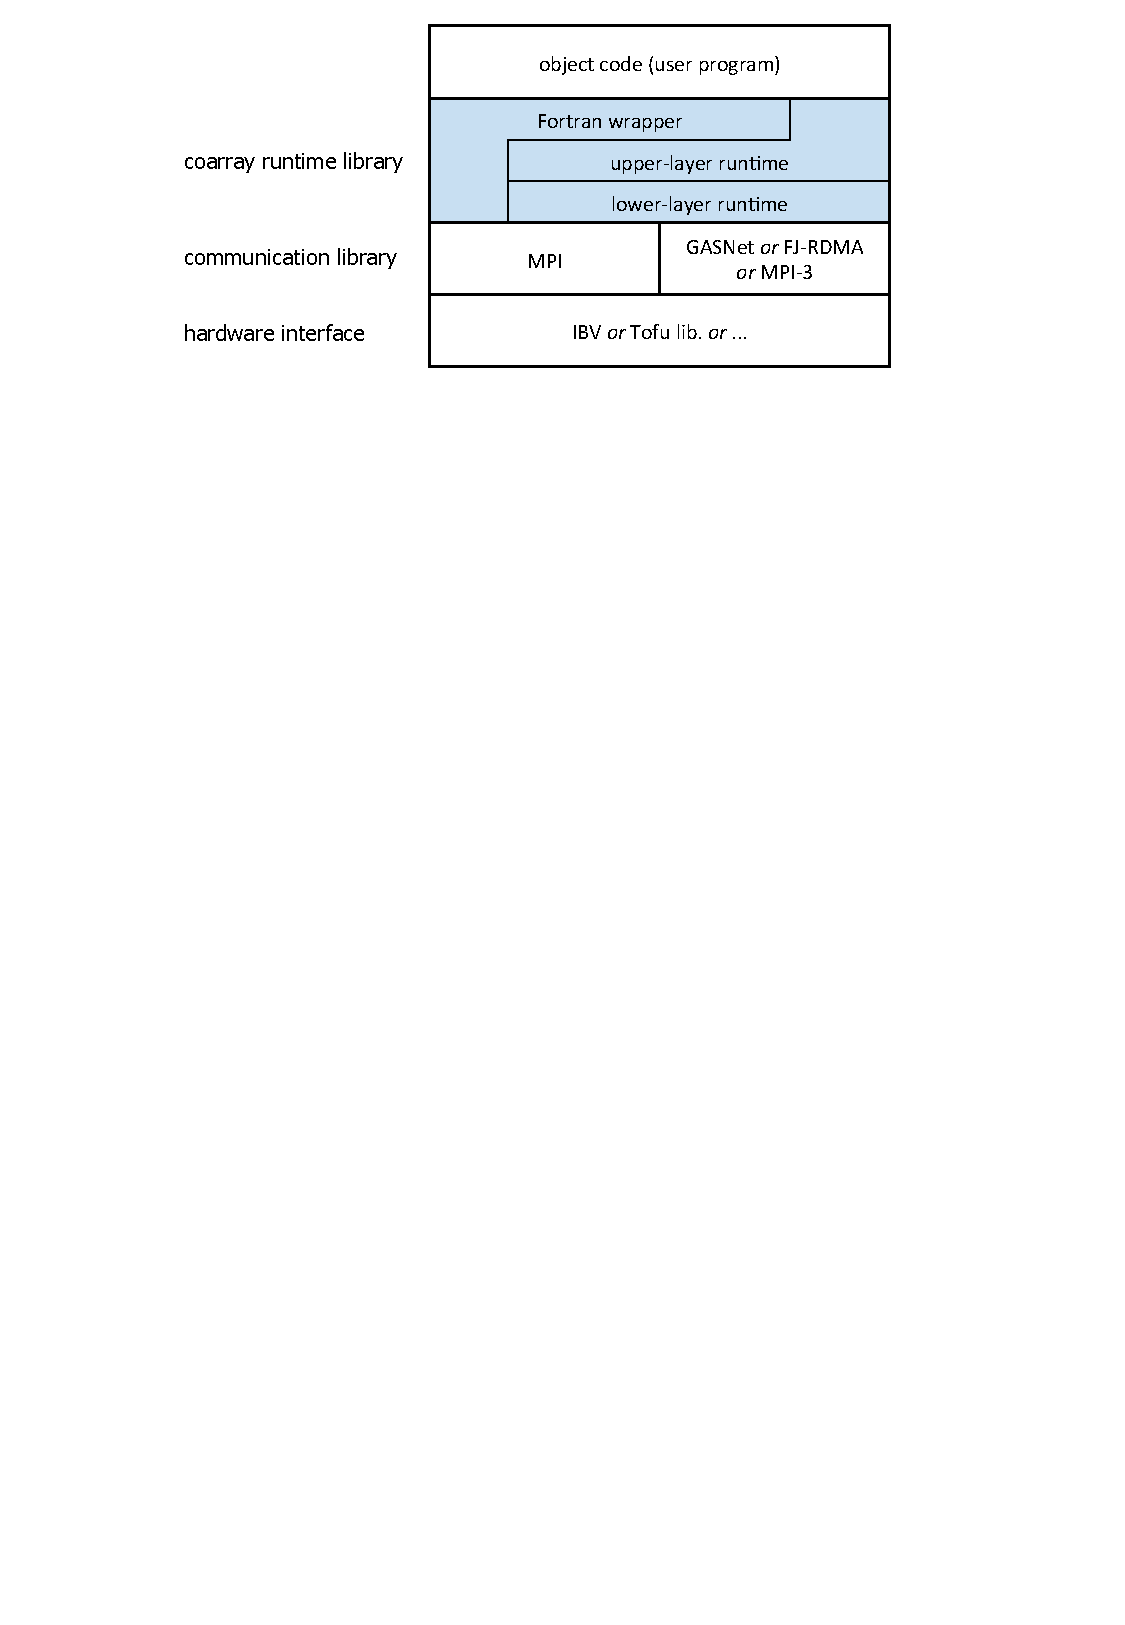
\includegraphics[trim=27mm 208mm 29mm 0mm, scale=0.7,clip]{figs/softstack-r4.pdf}}
    \caption{Software stack for coarray features}\label{fig:layer}
  \end{center}
\end{figure}


%===========================================================
\subsubsection{Fortran Wrapper}
%===========================================================

Each set of Fortran wrapper procedures has a generic name and dozens of corresponding specific names. For example, the object code contains a call to a function with
the generic name {\tt xmpf\_coarray\_get\_generic}.
If the data is a two-dimensional array of the 16-byte complex type,
the Fortran compiler selects the corresponding specific name 
{\tt xmpf\_coarray\_get2d\_z16} at compile time
and generates the object code by calling a ULR function 
by the specific name.

The Fortran wrapper accepts Fortran array notations as the arguments 
and the result variable and converts these notations into structures that can be handled in a runtime library written in C.
%
The Fortran wrapper also converts a C pointer to a Fortran pointer with the shape using
the Cray pointer.

The Fortran wrapper calls ULR procedures basically and 
calls MPI library functions directly for collective communications. 


%本実装では、Fortranの高級な仕様(配列記述や総称名手続き)を
%runtime libraryインタフェースとした。
%これにより、コンパイラが生成すべきオブジェクトインタフェースの数を
%数十分の一に削減してデータの型と形状をruntimeに伝えることができる
%ようになった。


%Actually, the interface is used through the Fortran~90 generic interface
%to ease the code generation by the coarray translator.
%For example, let us convert an {\tt ALLOCATE} statement
%{\tt allocate (a(1:10,2:19))}, where {\tt a} is an allocatable coarray of 16-byte,
%using object-ULR interface {\tt XMPCO\_malloc\_coarray}.
%The translator may generate a call to the generic procedure \\
%{\tt xmpf_coarray_malloc_generic(descriptor_of_a, a, 


%===========================================================
\subsubsection{Upper-layer Runtime (ULR) Library }
%===========================================================

The major role of ULR is performing the algorithms for coarray data
allocation/registration (\Sec{alloc}) and PUT/GET communications (\Sec{putget}).
Additionally, for atomic communications caused by intrinsic subroutines
{\tt ATOMIC\_DEFINE} and {\tt ATOMIC\_REF}, 
ULR calls the corresponding function of LLR after address calculation.

%===========================================================
\subsubsection{Lower-layer Runtime (LLR) Library}
%===========================================================

The LLR basically abstracts the difference between the communication libraries.
The only exception is the allocation and registration of coarray data.
Major functions are shown below.

\begin{itemize}
\item
Functions to allocate and register coarray variables,
and functions to register coarray variables that are already allocated.
They are alternatively used in the RS and RA methods and in the CA method.
Correspondingly, a set of functions to deregister and deallocate and
a set of functions to deregister are provided.

\item
Fundamental functions for RDMA-DMA GET communication and DMA-RDMA PUT communication.
It is assumed that both remote and local data are previously registered.
Blocking and non-blocking can be switched.
% and the only way to wait for
% the completion of the non-blocking communication is using the function
%corresponding to {\tt SYNC MEMORY}.

\item
Functions corresponding to image control statements, atomic subroutines,
and inquire functions.

\end{itemize}

The LLR also has the features for multi-dimensional data developed for the C 
implementation, which are not used in the Fortran implementation because
this implementation is solved in ULR.


%===========================================================
\subsubsection{Communication Libraries}
%===========================================================

MPI-3 can be selected for all platforms on which it is implemented. Coarrays are 
registered and deregistered at the start and end point of the MPI window. 
Coarrays perform one-sided communication by {\tt MPI\_Put} and {\tt MPI\_Get}
and are synchronized by {\tt MPI\_Win\_fence}. 
Implementation on MPI incurs certain costs for dynamic allocation of coarrays and 
waiting for communication completion.

GASNet can be selected for more advanced implementation over InfiniBand. 
Since allocation and registration of are inseparable and can be performed only once 
on GASNet, the implementation allocates and registers a pool of memory,
the size of which should be large enough to contain all static and allocatable coarrays.
The XMP runtime should allocate and deallocate coarrays without using the Fortran 
library but using the memory manager constructed for the pool.

FJ-RDMA can be selected for the implementation over the Tofu interconnection of 
the K computer and Fujitsu PRIMEHPC FX series supercomputers. 
Basically, each coarray is allocated by the Fortran library and 
the address is registered with the FJ-RDMA interface {\tt FJMPI\_Rdma\_reg\_mem}. 
The address is deregistered with {\tt FJMPI\_Rdma\_dereg\_mem} before being deallocated 
(freed) by the Fortran library. 
One-sided communication is performed with {\tt FJMPI\_Rdma\_put} and 
{\tt FJMPI\_Rdma\_get}.
%, which include confirmation of communication completion. <-- 本当? いつも?





%\cleardoublepage

\section{Evaluation}\label{sec:eval}

We evaluated the Omni coarray compiler on the systems shown in \tab{specs}.

\begin{table}
 \begin{center}
  \caption{Specs of the compulters used for evaluation}\label{tab:specs}
  \begin{tabular}{l|p{0.4\textwidth}|p{0.4\textwidth}}
   \hline
   & HOKUSAI GreatWare (RIKEN RCCS)   & CCS, University of Tsukuba \\
   & Fujitsu PRIMEHPC FX100           & HA-PACS/TCA \\
   \hline
   \hline
   CPU
   & SPARK64\texttrademark XIfx, 1.975GHz, 1CPU per node, 4-SIMD $\times$ 32-core
   & E5-2680 v2 (Ivy Bridge), 10-core, 224GFlops, 2CPU per node \\
   \hline
   memory
   & 32GB per node, bandwidth 480GB/s per node
   & DDR3 SDRAM 128GB per node, 119.4GB/s   \\
   \hline
   interconnect
   & Tofu2, 12.5GB/s $\times$ 2
   & InfiniBand FDR, 7GB/s \\
   \hline
   compiler
   & Fujitsu Fortran Ver.\ 2.0.0 P-id:T01776-01
   & Intel Fortran 16.0.4 \\
   \hline
   MPI
   & Fujitu MPI Ver.\ 2.0.0 P-id:T01776-01 (OpenMPI base)
   & Intel MPI 5.1.3 \\
   \hline
   comm.\ layer
   & Tofu library
   & GASNet 1.24.2 built as IBV-conduit with Intel compilers \\
   \hline
  \end{tabular}
 \end{center}
\end{table}



%-----------------------------------------------------------------------------
\subsection{Fundamental Performance}
%-----------------------------------------------------------------------------

%===============
% 説明
%===============

Using EPCC Fortran Coarray micro-benchmark~\cite{EPCC}, we evaluated ping-pong performance 
of PUT and GET communications compared with MPI\_Send/Recv.
The codes are shortly shown in \tab{pingpong-code}.

%-- pingpong-code.pdf
\begin{table}[bht]
  \begin{center}
    \caption{pingpong-code.pdf}\label{tab:pingpong-code}
    % trimはleft bottom right topの順
    \mbox{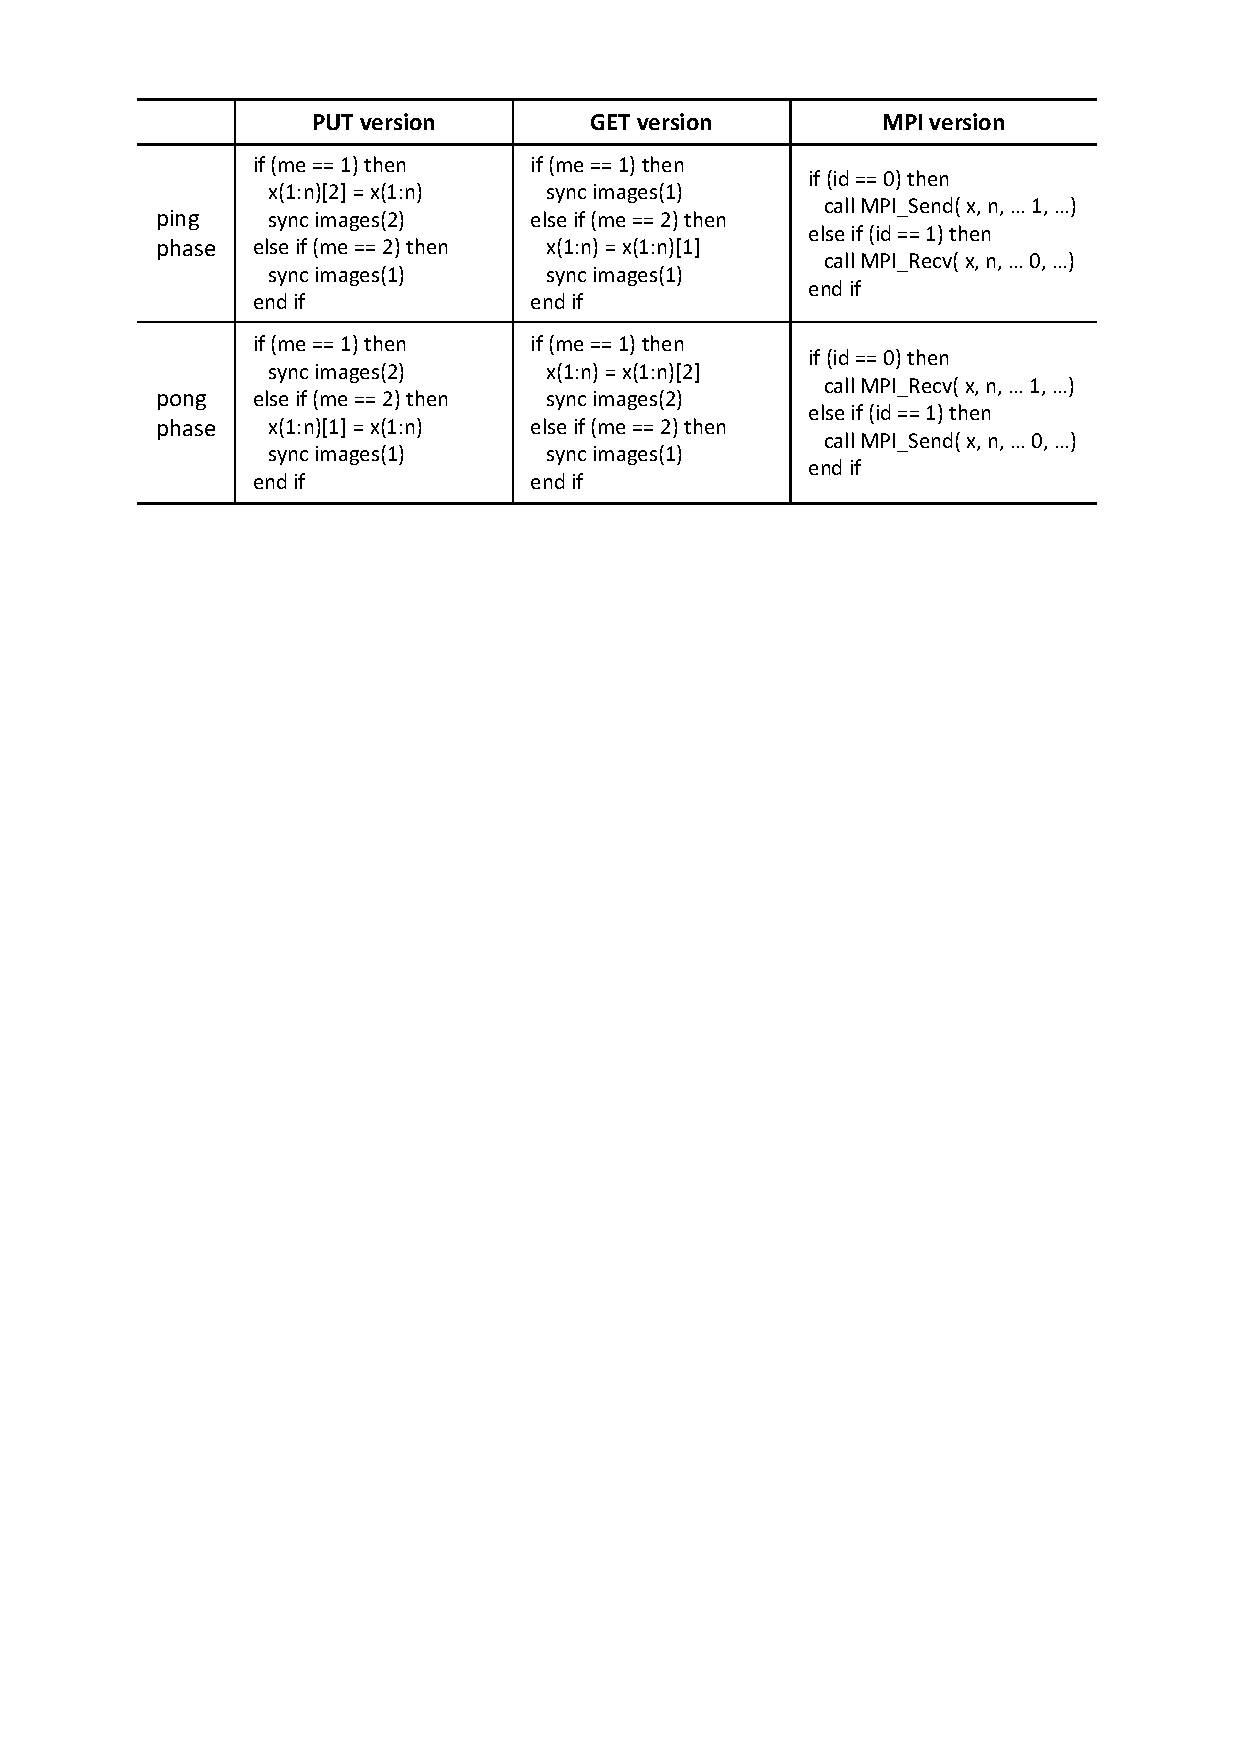
\includegraphics[trim=24mm 211mm 24mm 16mm, scale=0.7,clip]{figs/pingpong-code-r2.pdf}}
    \begin{flushright}
      {\tt me} is the image index. {\tt id} is the MPI rank number.
    \end{flushright}
  \end{center}
\end{table}

%-- pingpong-fig.pdf
\begin{figure}[bht]
  \begin{center}
    \mbox{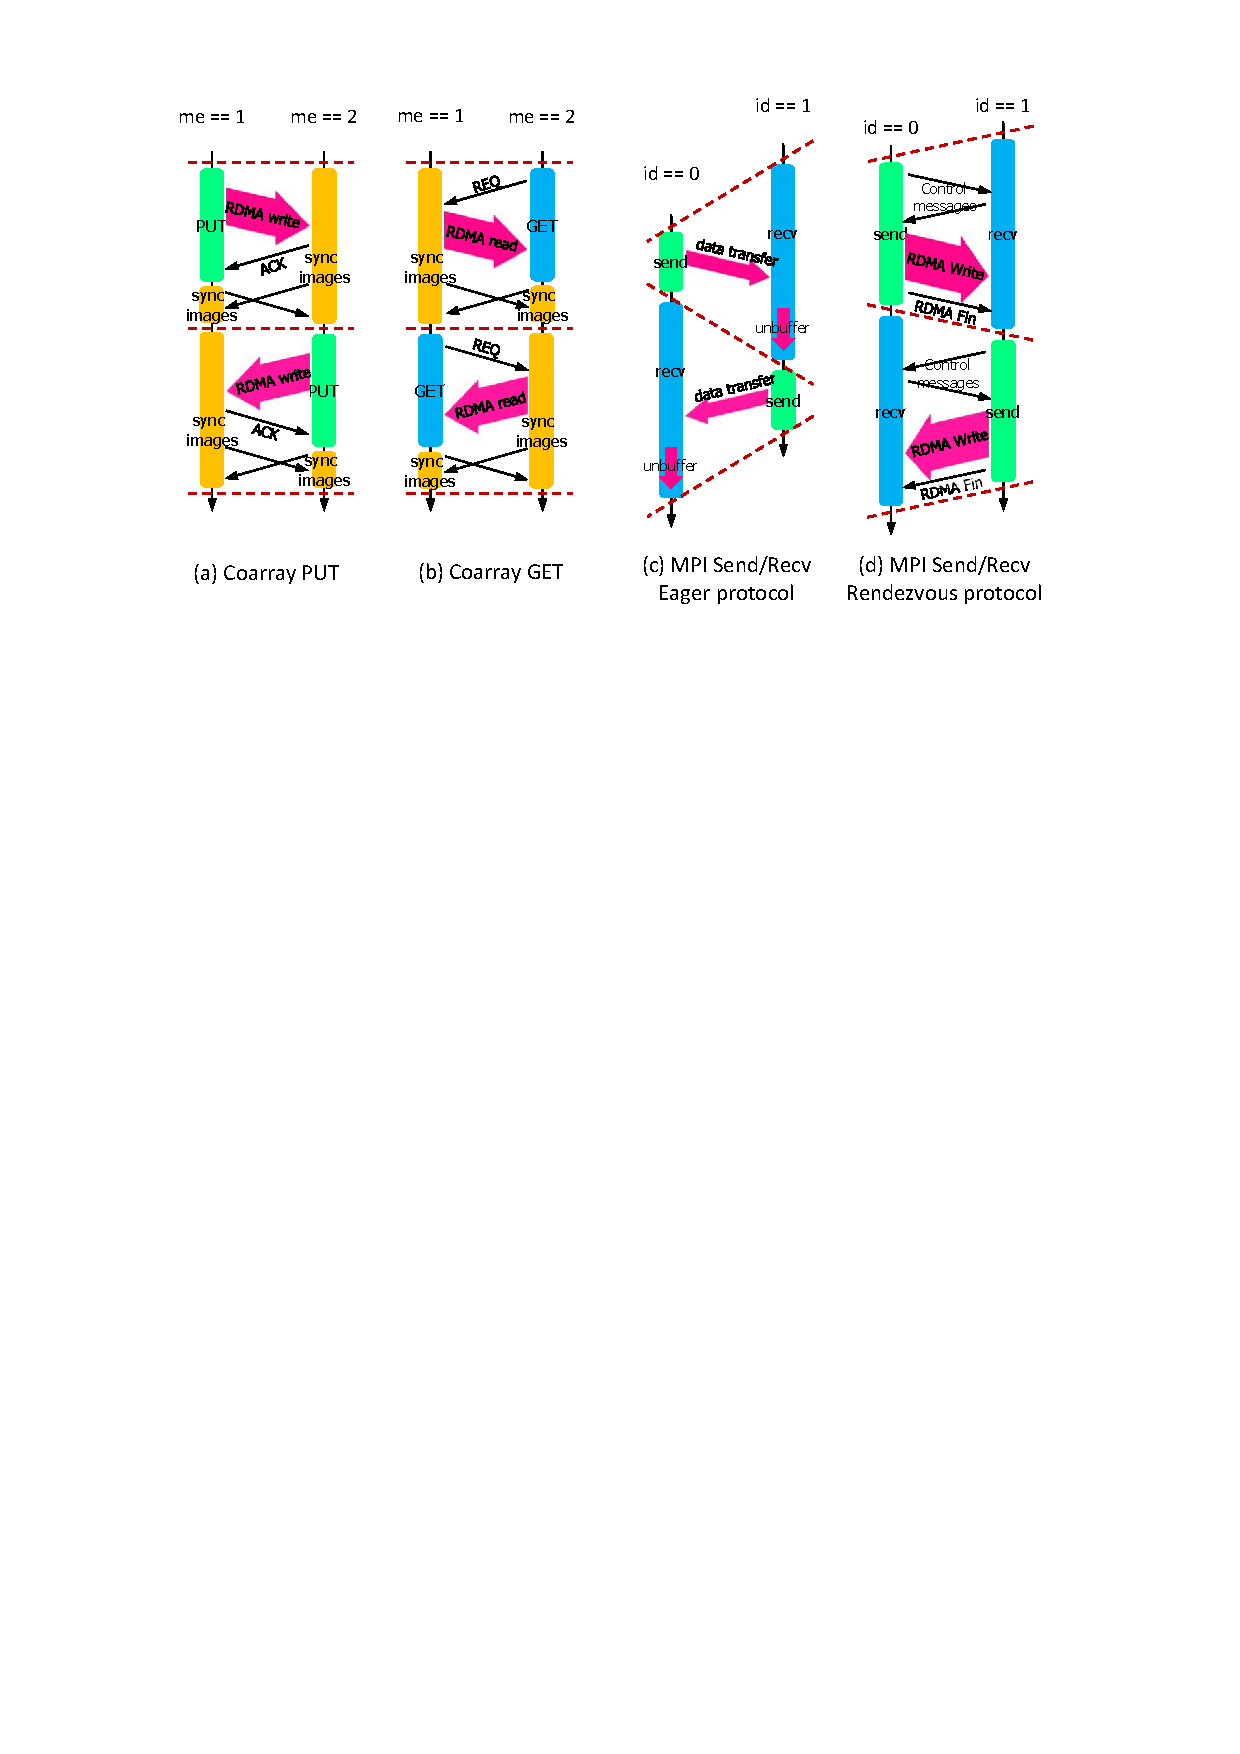
\includegraphics[trim=30mm 195mm 32mm 16mm, scale=0.75,clip]{figs/pingpong-fig-r2.pdf}}
    \caption{pingpong-fig.pdf}\label{fig:pingpong-fig}
  \end{center}
\end{figure}

Corresponding to the codes in \tab{pingpong-code}, \fig{pingpong-fig} shows how data and 
messages are echanged between two images or processes.
In coarray PUT (a) and GET (b), inter-image synchronization is necessary for each end of 
phases to make the passive image active and to make the active image passive.
While, in MPI message-passing (c) and (d), such synchronization is not necessary because
both processes are always active.
%
On the other hand, MPI message-passing has its own overhead that coarray PUT/GET
does not have. Because the eager protocol (c) does not use RDMA, the receiver
must copy the received data in the local buffer to the target. The larger the data,
the greater the overhead cost.
In the rendezvous protocol (d), negotiations including remote address notification
are required prior to the communication.
The overhead cost is not negligible when the data is small.


%===============
% 結果
%===============

\begin{figure}[p]
  \begin{center}
    % trimはleft bottom right topの順
    %\mbox{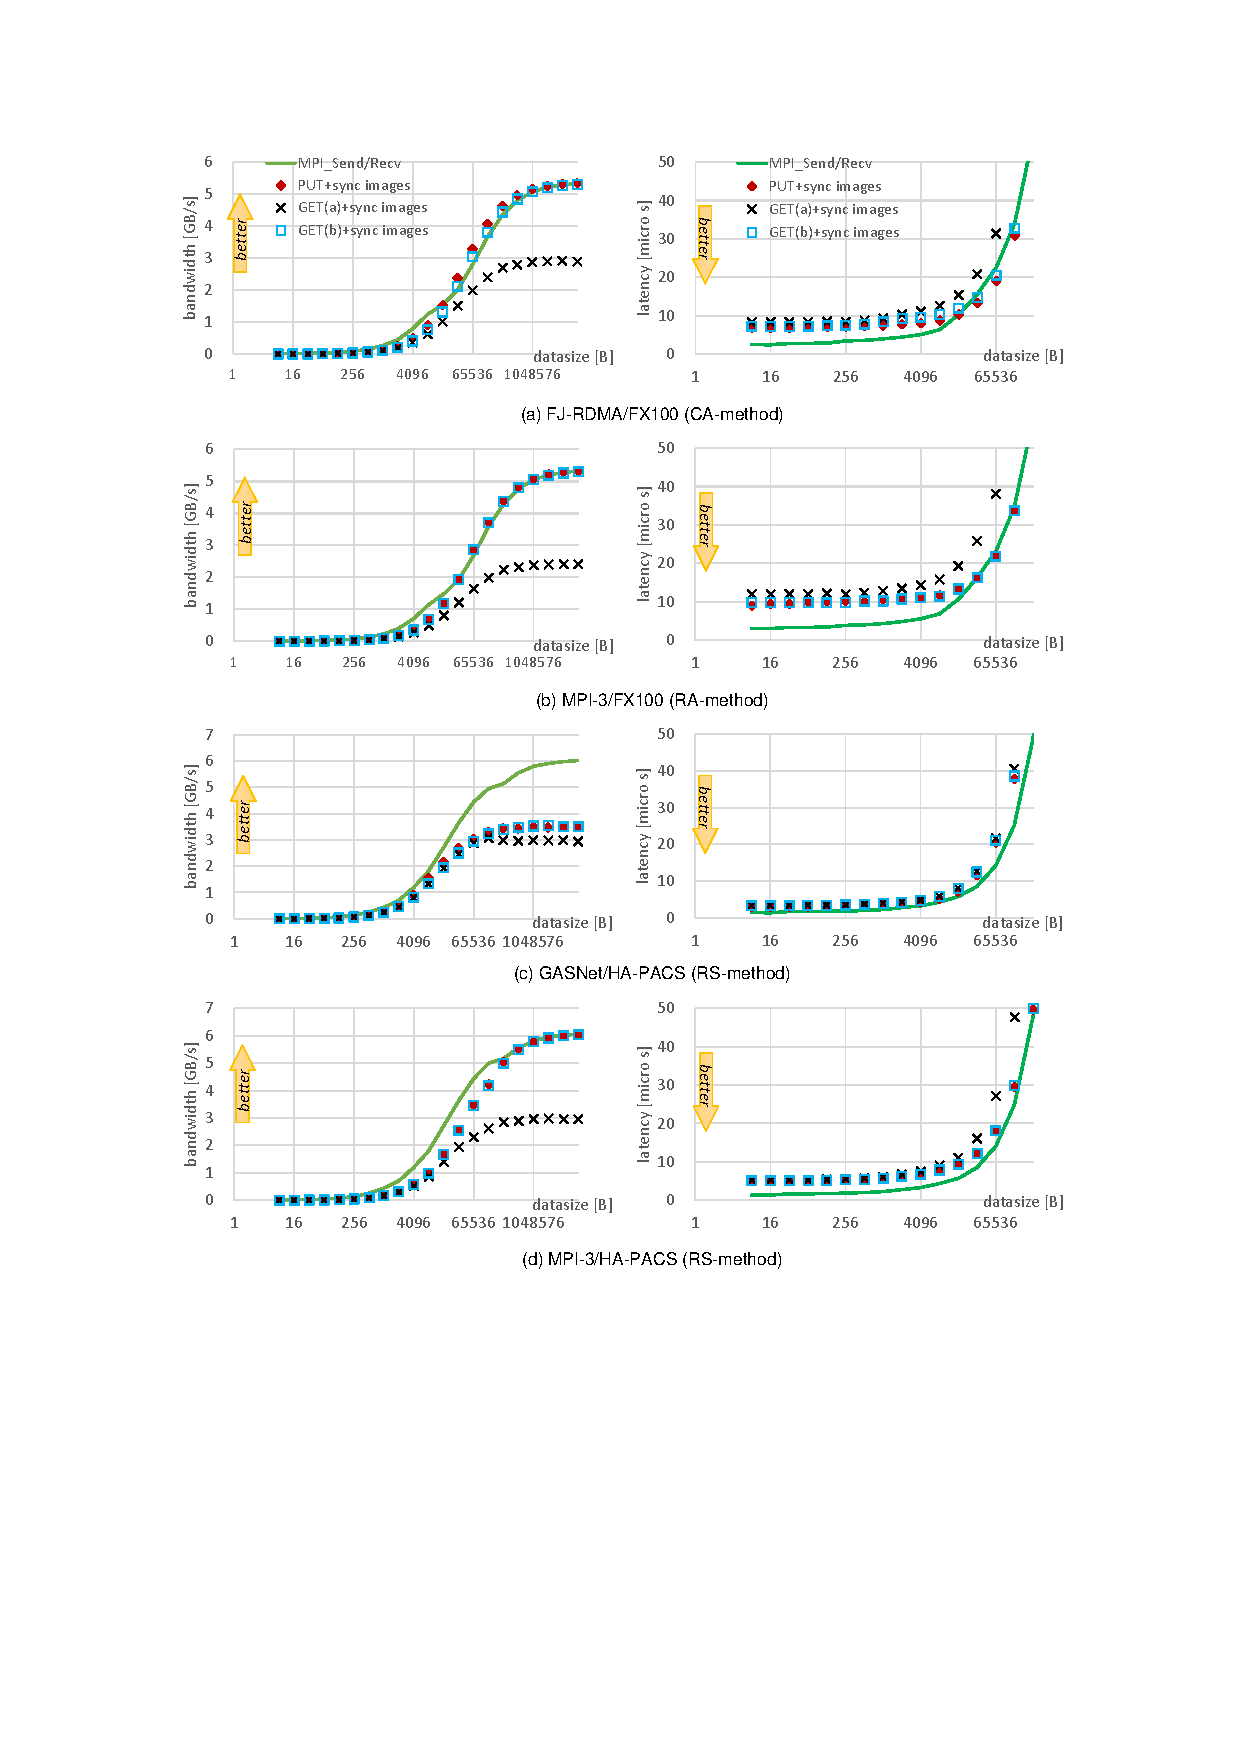
\includegraphics[trim=30mm 80mm 30mm 25mm, scale=0.8, clip]{graphs/8graphs-7.pdf}}
    \mbox{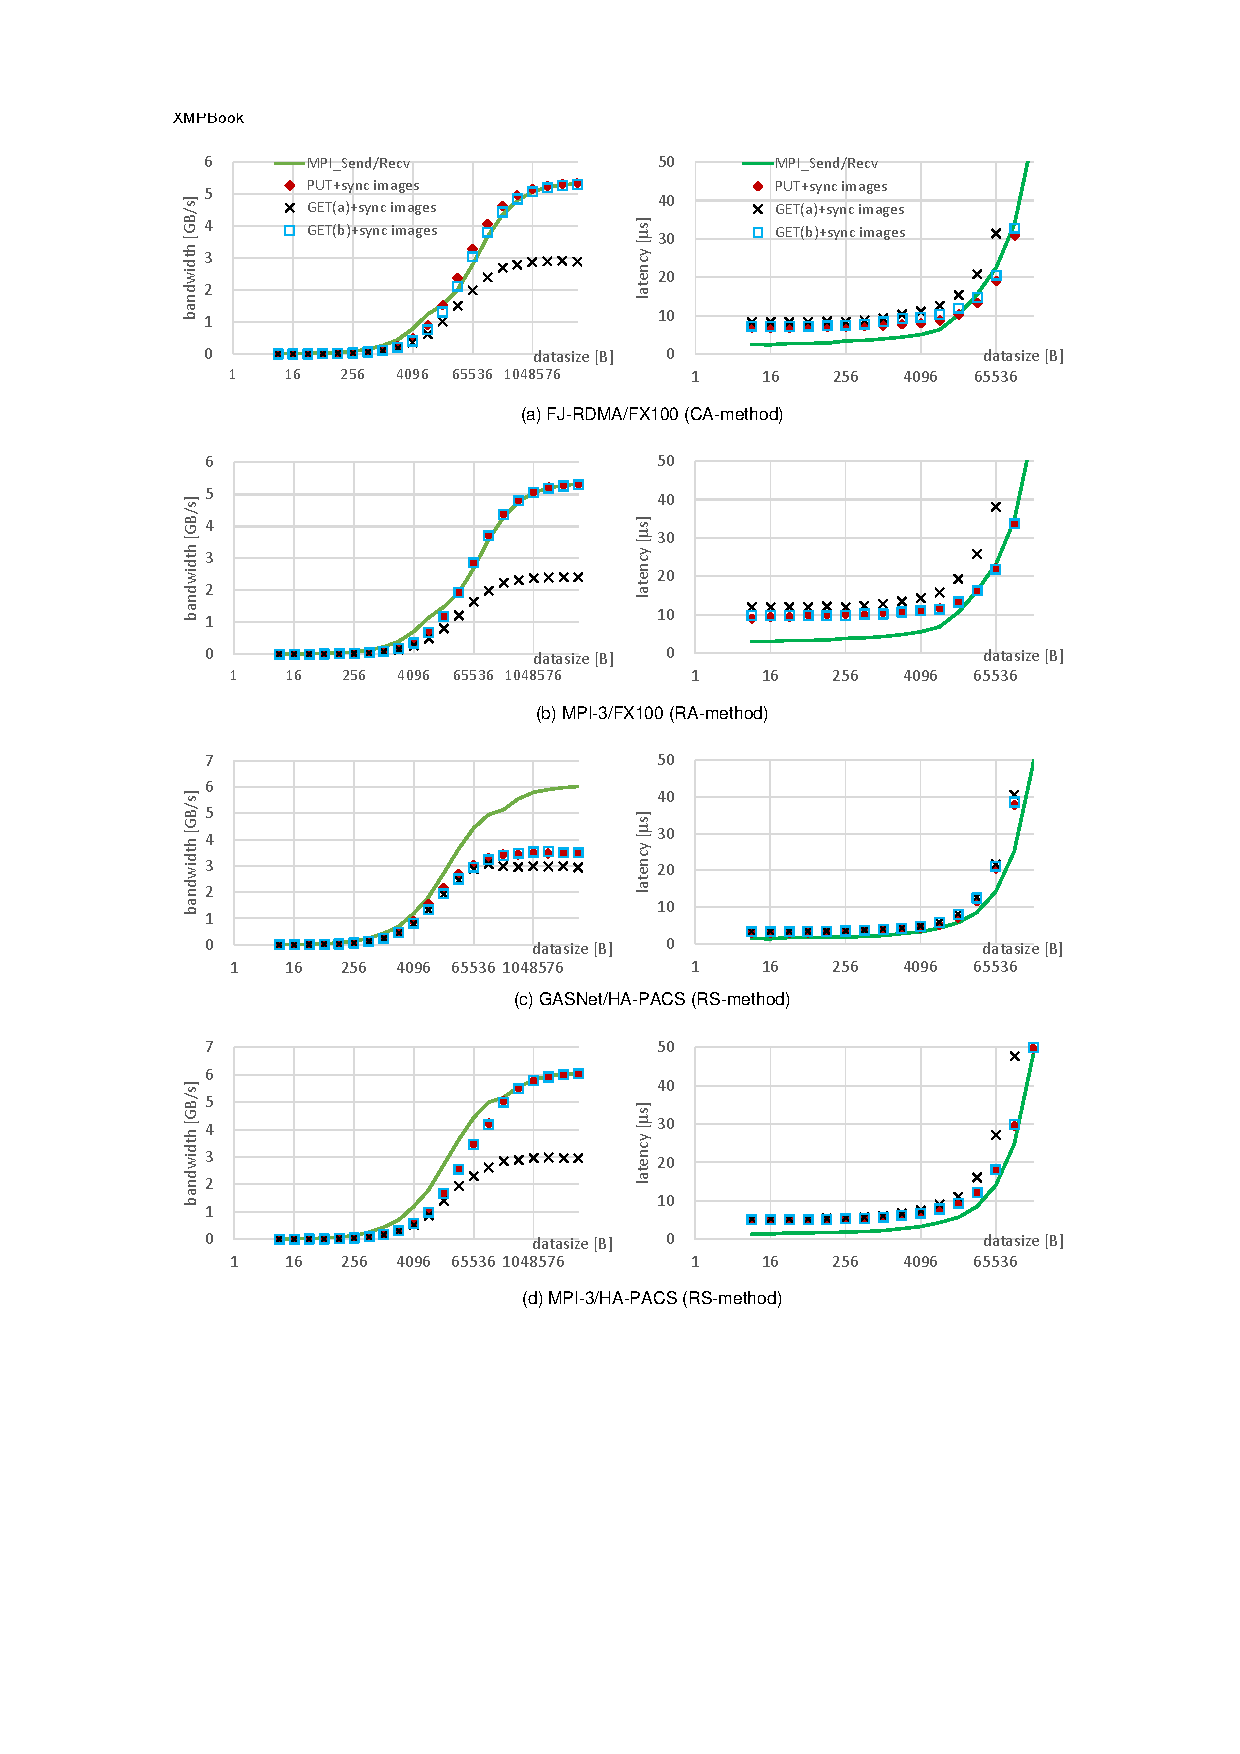
\includegraphics[trim=30mm 70mm 30mm 23mm, scale=0.78, clip]{graphs/8graphs-8.pdf}}
    \caption{Ping-pong performance on Fujitsu PRIMEHPC FX100 and HA-PACS/TCA}\label{fig:8graphs}
  \end{center}
\end{figure}

The result of the comparision between coarray PUT/GET and MPI message passing is shown in
\fig{8graphs}.
As the underlying communication libraries, 
FJ-RDMA and MPI-3 are used on FX100 and GASNet and MPI-3 are used on HA-PACS.
GET(a) and GET(b) are using the code without and with the optimization described in
\Sec{opt-get}, respectively.
Bandwidth is the communication data size per elapsed time, and
latency is half of the ping-pong elapsed time.
The difference between GET(a) and (b) is the compile-time optimization level of the 
coarray translator described in \Sec{opt-get}.

%===============
% 分かったこと
%===============

As the result, the following was found about coarray PUT/GET communication.

\begin{enumerate}

\item {\em Bandwidth.}
Coarray PUT and GET are slightly outperforms MPI rendezvous communication for large data 
on FJ-RDMA and MPI-3.
On FJ-RDMA/FX100 (a), the bandwidth of PUT and GET(b) are respectively 
+0.1\% to +18\% and -0.4\% to +9.3\% higher than MPI rendezbous in the 
rendezvous range of 32k through 32M bytes.
Also on MPI-3/HA-PACS, respectively +0.3\% to +0.8\% and 
+0.1\% to +1.3\% higher in the rendezvous range of 512k through 32M bytes.

It was confirmed from the runtime log that zero-copy communication was performed
both in PUT and GET(b) by selecting DMA scheme described in \Sec{opt-dma}.

However, on GASNet/HA-PACS (c), PUT and GET(b) has only about 60\% bandwidth for large data
than MPI rendezvous.
It is presumed that data copy was caused internally.

\item {\em Latency.}
On FJ-RDMA (a) and MPI-3 (b) and (d), PUT and GET(b) have larger (worse) latency than 
MPI eager communication, in the range of $\leq$16kB on FX100 and $\leq$256kB on HA-PACS.

Coarray on GASNet (c) behaves differently than other cases on (a), (b) and (d).
Though the latency is larger than the one of MPI for all data sizes, the difference
is smaller than the other cases. At data size 8B, the latency of PUT is 2.93$\mu$s
and 2.1 times larger than the one of MPI 
while 5.73$\mu$s and 3.7 times larger on the case of MPI-3 (d).

\item {\em Effect of GET optimization.}
For all ranges of all cases, GET(a) has smaller bandwidth and larger latency than GET(b).
On FJ-RDMA (a), the bandwidth is 1.41 to 1.85 times improved in the range of 32kB to 32MB
by changing the object code of GET(a) to (b).
We found GET(a) caused two extra memory copies; one is performing the array assignment 
by the Fortran library and the other is the copy from the communication buffer 
to the result variable of the array function {\tt xmpf\_coarray\_get\_generic}. 
The optimization described in \Sec{opt-get} has eliminated these two data copies.

\end{enumerate}

The issue is the large latency of coarray PUT/GET communication.
In the next subsection, it is discussed how it should be solved 
by the compiler and the programming.



%===========================================================
\subsection{Non-blocking communication}
%===========================================================

For latency hiding, asynchronous and non-blocking features can be expected 
on coarray PUT communication.
The principle is shown in \fig{nonblock-fig}.
%
\fig{nonblock-fig} (a) illustrates the half pattern of the ping-pong PUT communication.
Coarray one-sided communication is basically asynchronous unless 
synchronization is explicitly specified. Therefore, multiple communications
without synchronization between them, as shown in (b), is closer to actural applications.
In addition, it can be optimized using non-blocking communication as shown in (c).
Blocking and non-blocking communications can be switched with the runtime environment
variable in the current implementation of the Omni compiler.
In MPI message passing, non-blocking communication can be written with 
{\tt MPI\_Isend}, {\tt MPI\_Irecv} and {\tt MPI\_Wait}.

%-- nonblock-fig.pdf
\begin{figure}[tbh]
  \begin{center}
  % trimはleft bottom right topの順
    \mbox{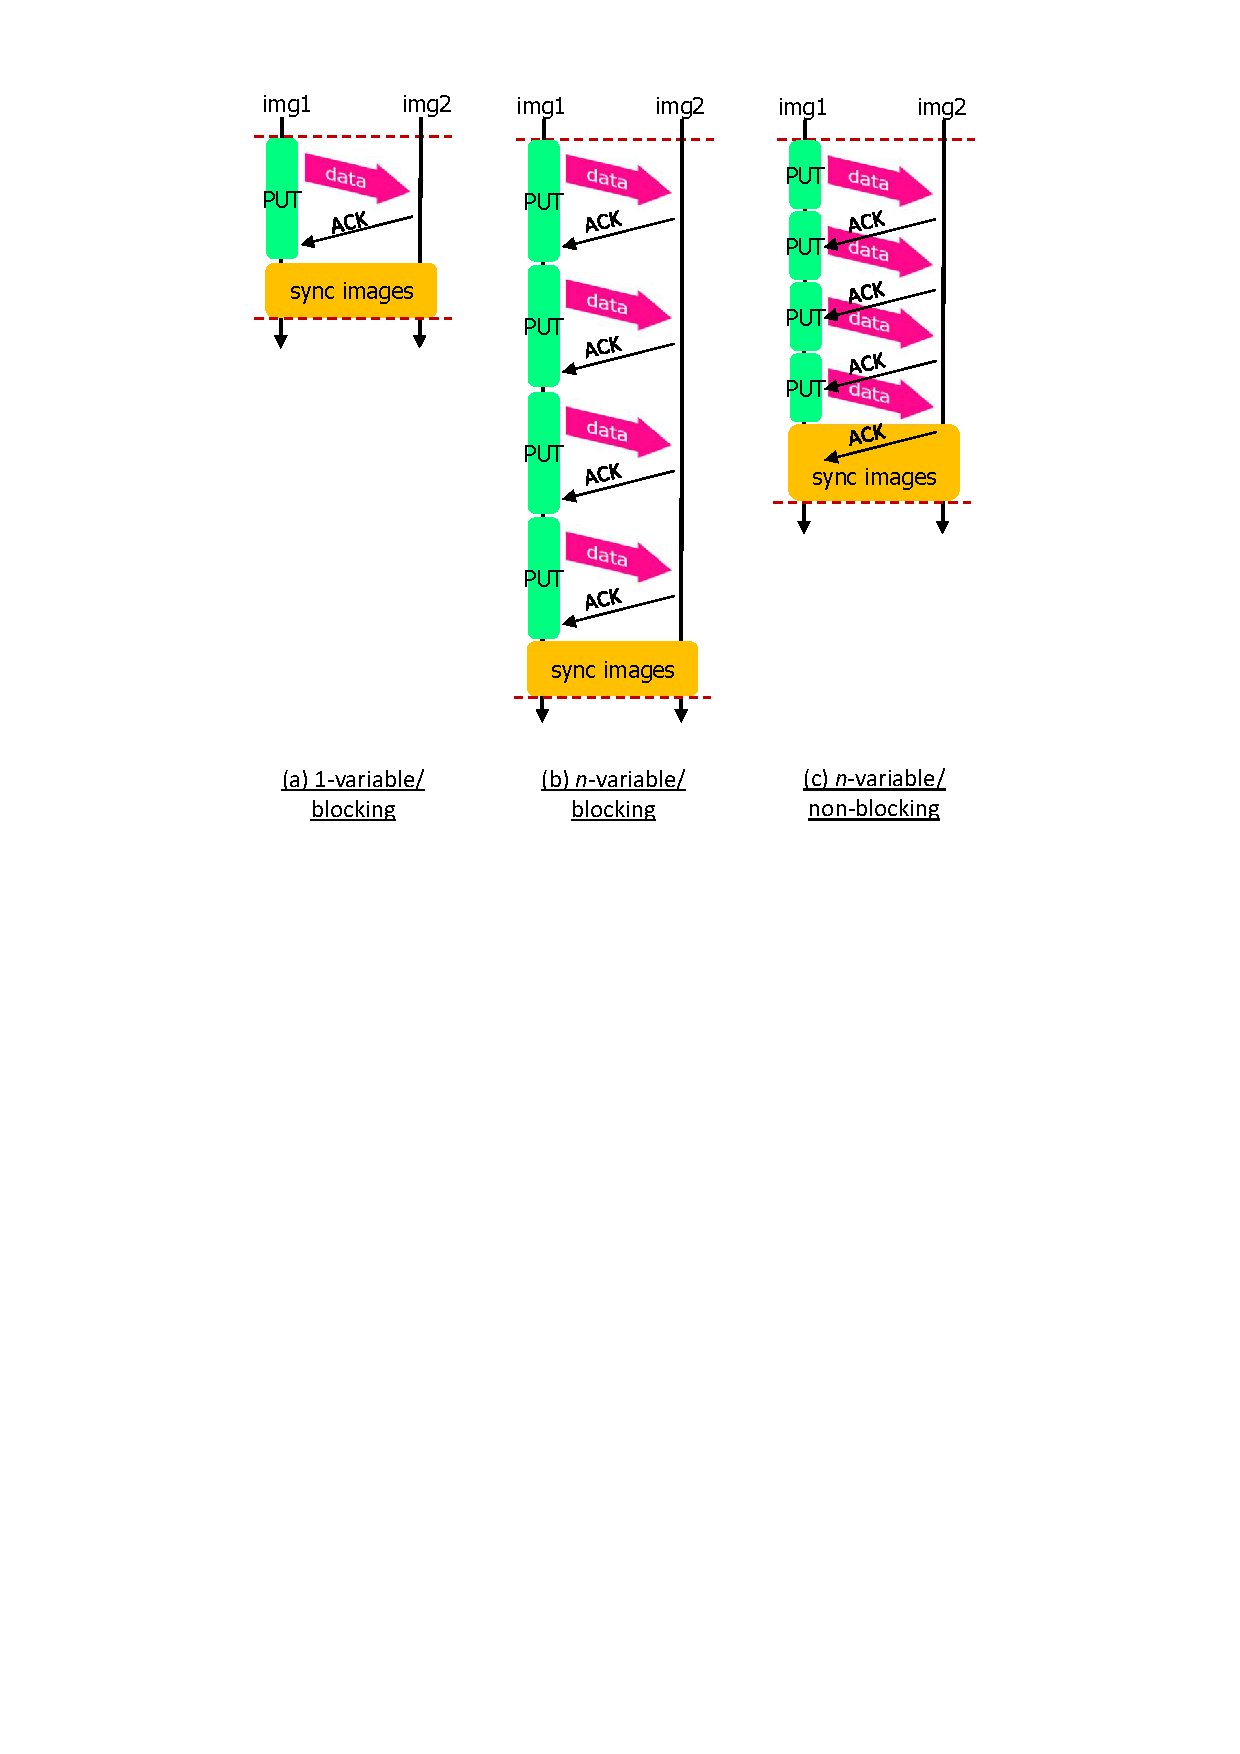
\includegraphics[trim=43mm 144mm 43mm 3mm, scale=0.6,clip]{figs/nonblock-fig-r2.pdf}}
    \caption{nonblock-fig.pdf}\label{fig:nonblock-fig}
  \end{center}
\end{figure}


\fig{8var-pingpong} compares blocking/non-blocking coarray PUT and 
MPI message passing communications.
Two original graphs are the same as the ones of \fig{8graphs} (a).
Other four graphs display the result of 8-variable ping-pong program, 
which repeats the ping phase sending eight individual variables 
from one to the other in order and the pong phase doing similarly 
in the opposite direction.
Each blocksize indicates the size of variables and latency includes the
time for eight variables.
%
The result shows that non-blocking has significantly improved the latency of 
PUT communication. 
Non-blocking PUT is 4.63 times faster than blocking PUT on average from 8B to 8kB. 
Compared to the original PUT, it performs 8 times the communication in just 
2.11 times longer on average from 8B to 8kB.
%
In MPI eager protocol, non-blocking has no effect for latency hiding.
As the result, 8-variable non-blocking PUT had lower or almost the same 
latency than blocking and non-blocking MPI message passing.
The ratio is up to 2.17 times at 8kB comparing to 8-variable blocking MPI.

\begin{figure}
  \begin{center}
    %-- 8var-pipo-latency.pdf
    %\mbox{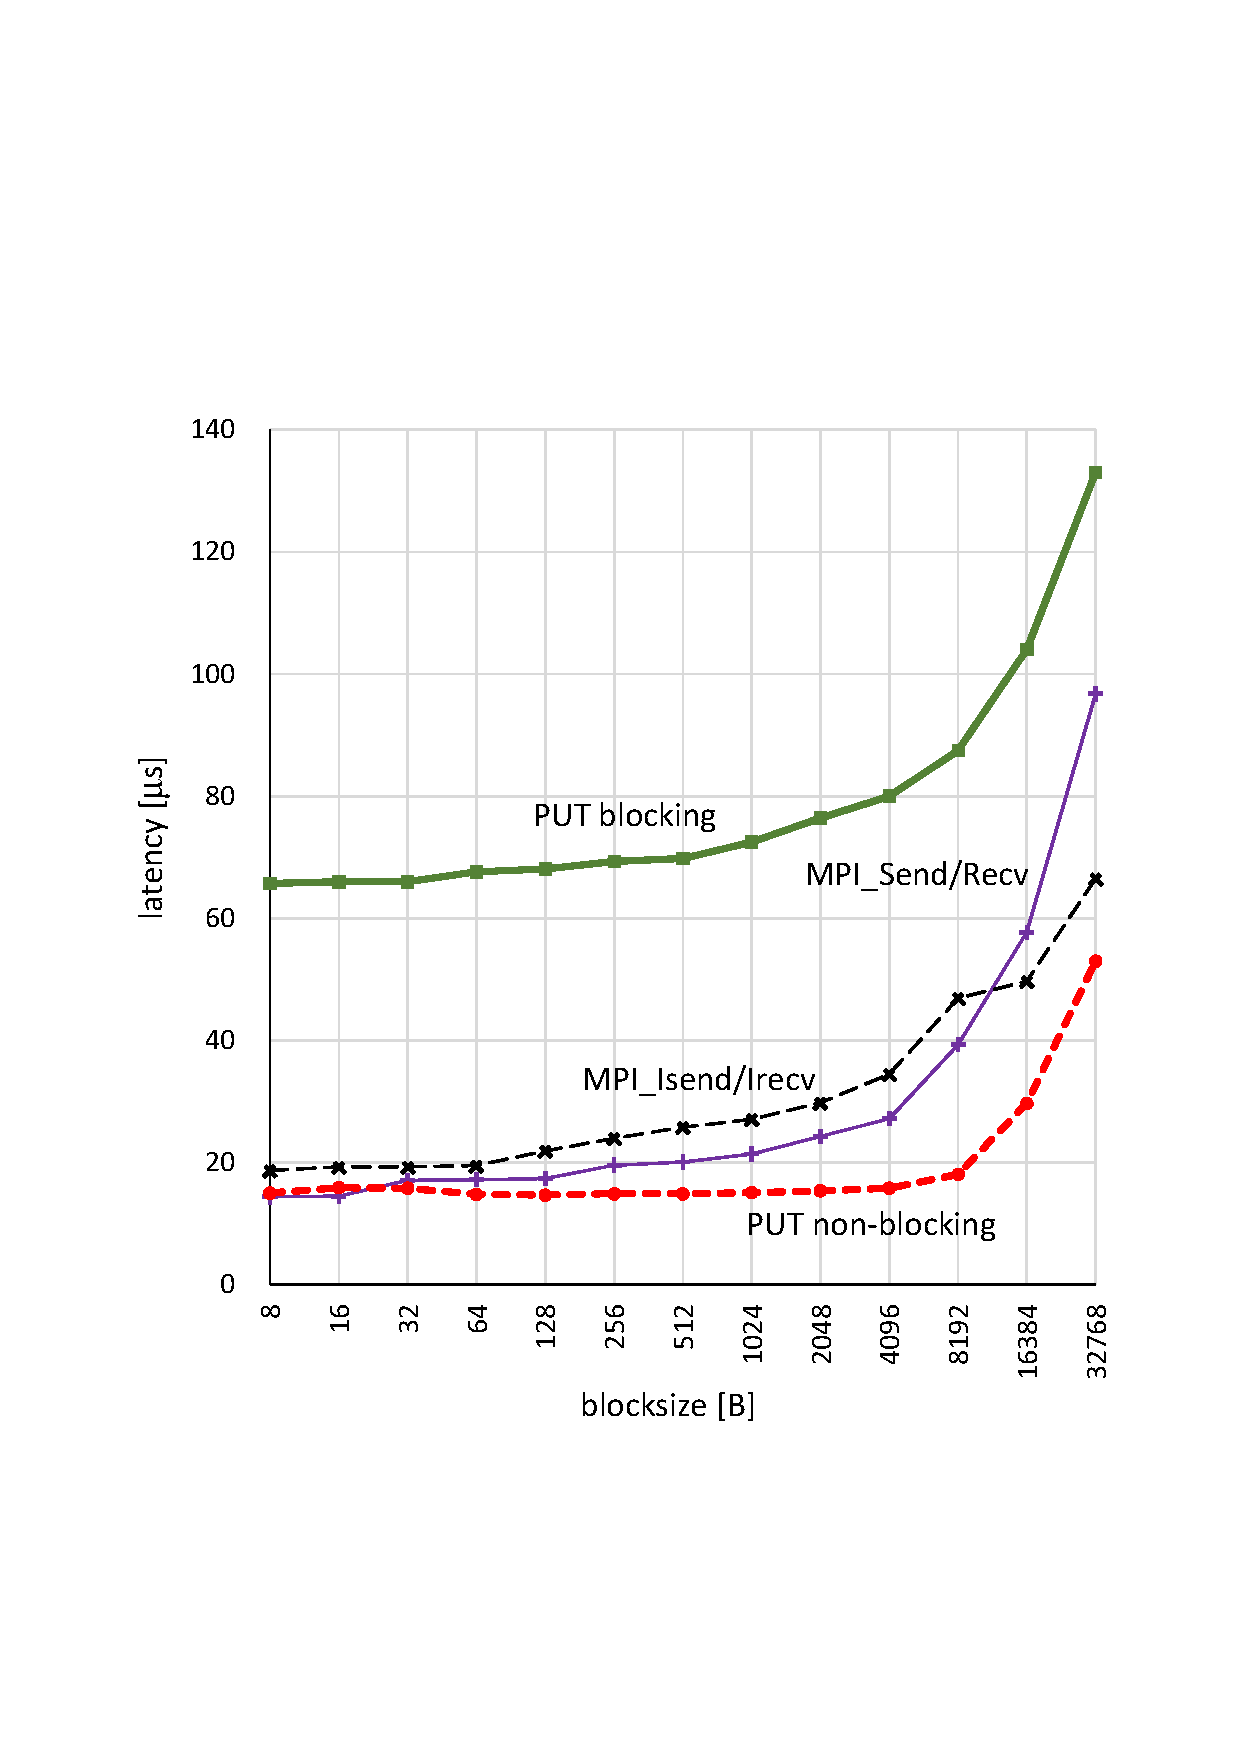
\includegraphics[trim=20mm 52mm 5mm 65mm,scale=0.45,clip]{graphs/8var-latency.pdf}}
    \mbox{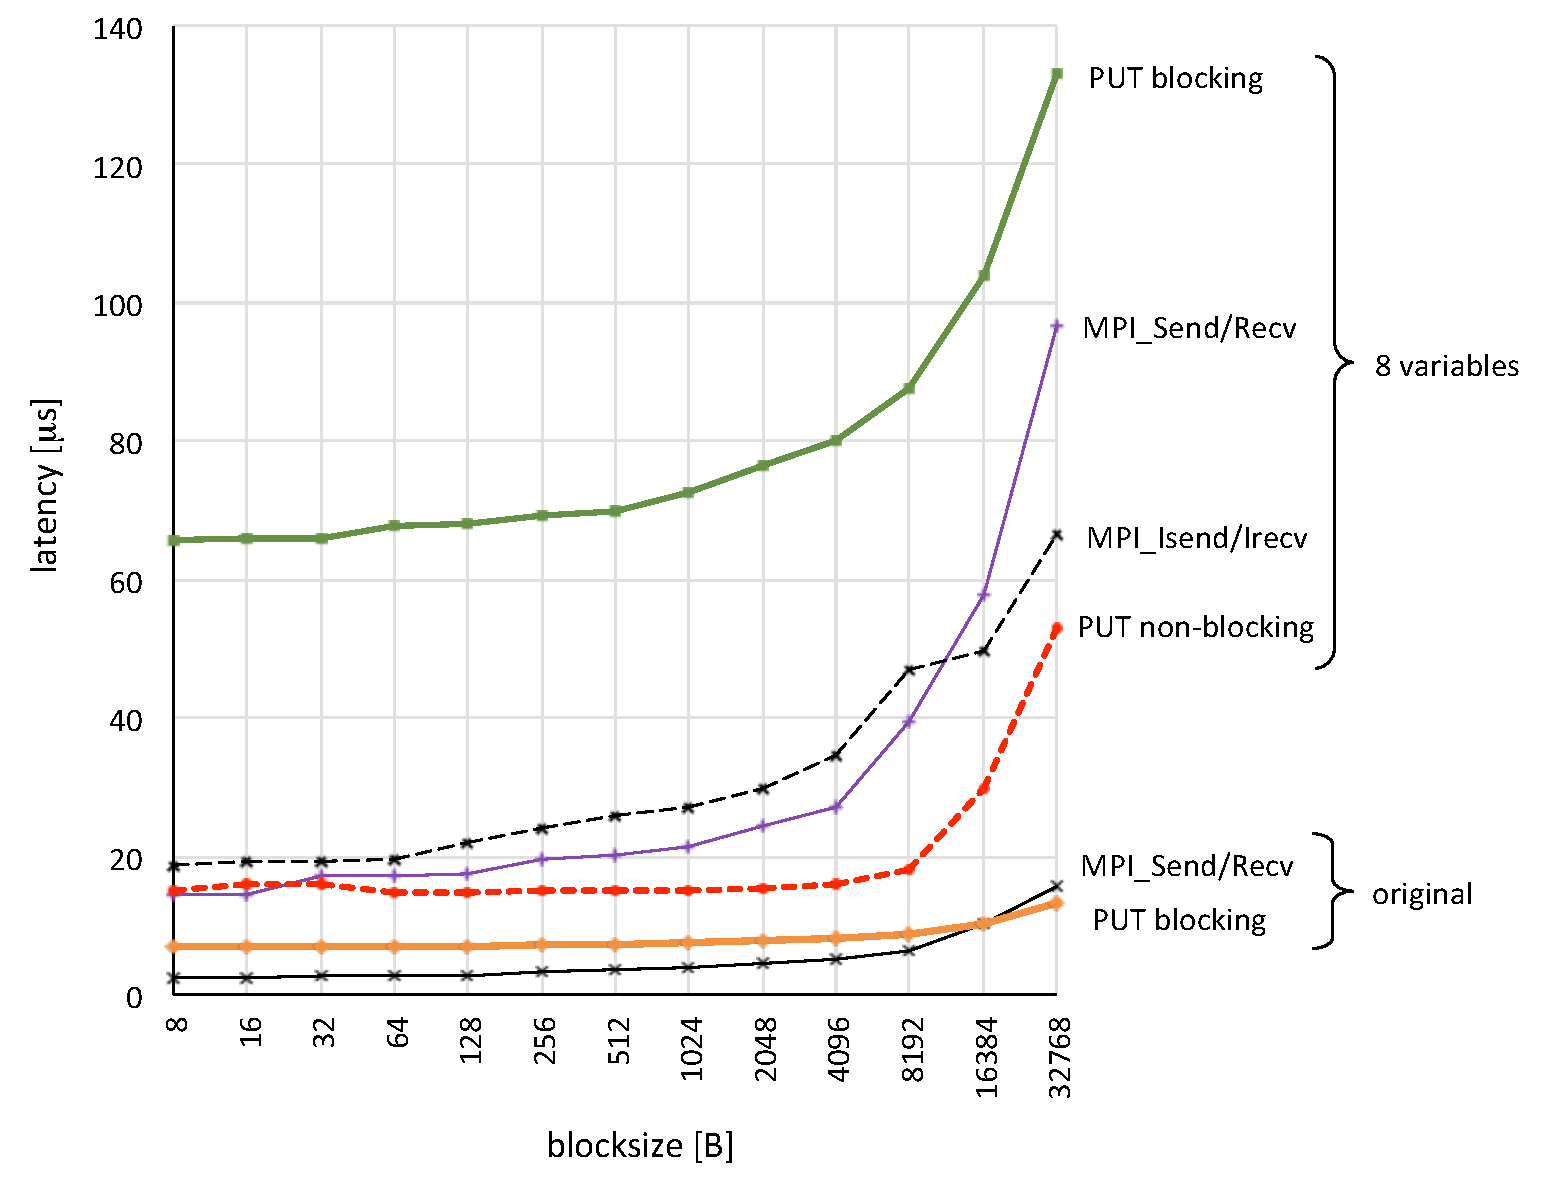
\includegraphics[scale=0.45]{graphs/8var-latency-2.pdf}}
    \caption{8-variable ping-pong latency on PRIMEHPC FX100}\label{fig:8var-pingpong}
   \end{center}
\end{figure}
    

%\begin{figure}
%  \begin{center}
%    %-- 8var-pipo-bw.pdf
%    \mbox{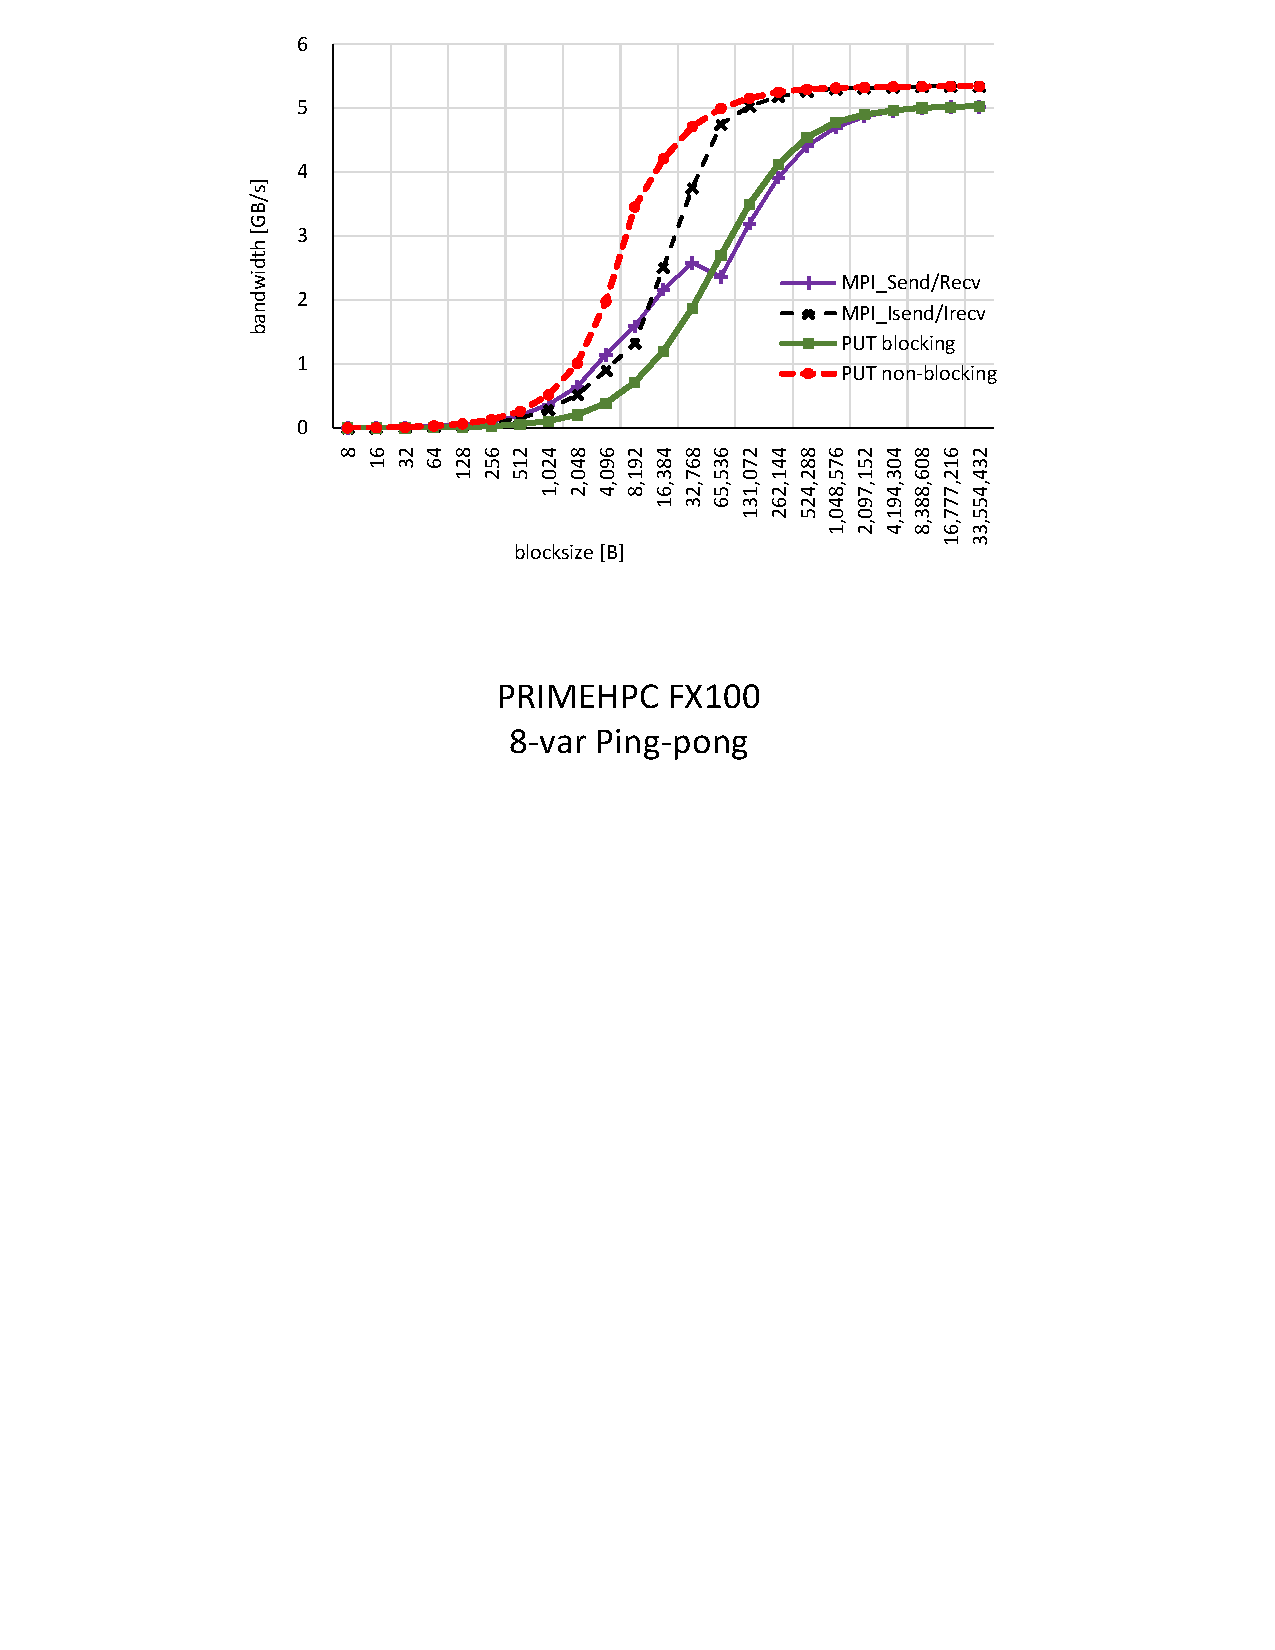
\includegraphics[trim=40mm 180mm 43mm 0mm, scale=0.6,clip]{figs/8var-pipo-bw.pdf}}\\
%    (a) Bandwidth of blocking and non-blocking communications\\
%    %-- 8var-pipo-latency.pdf
%    \mbox{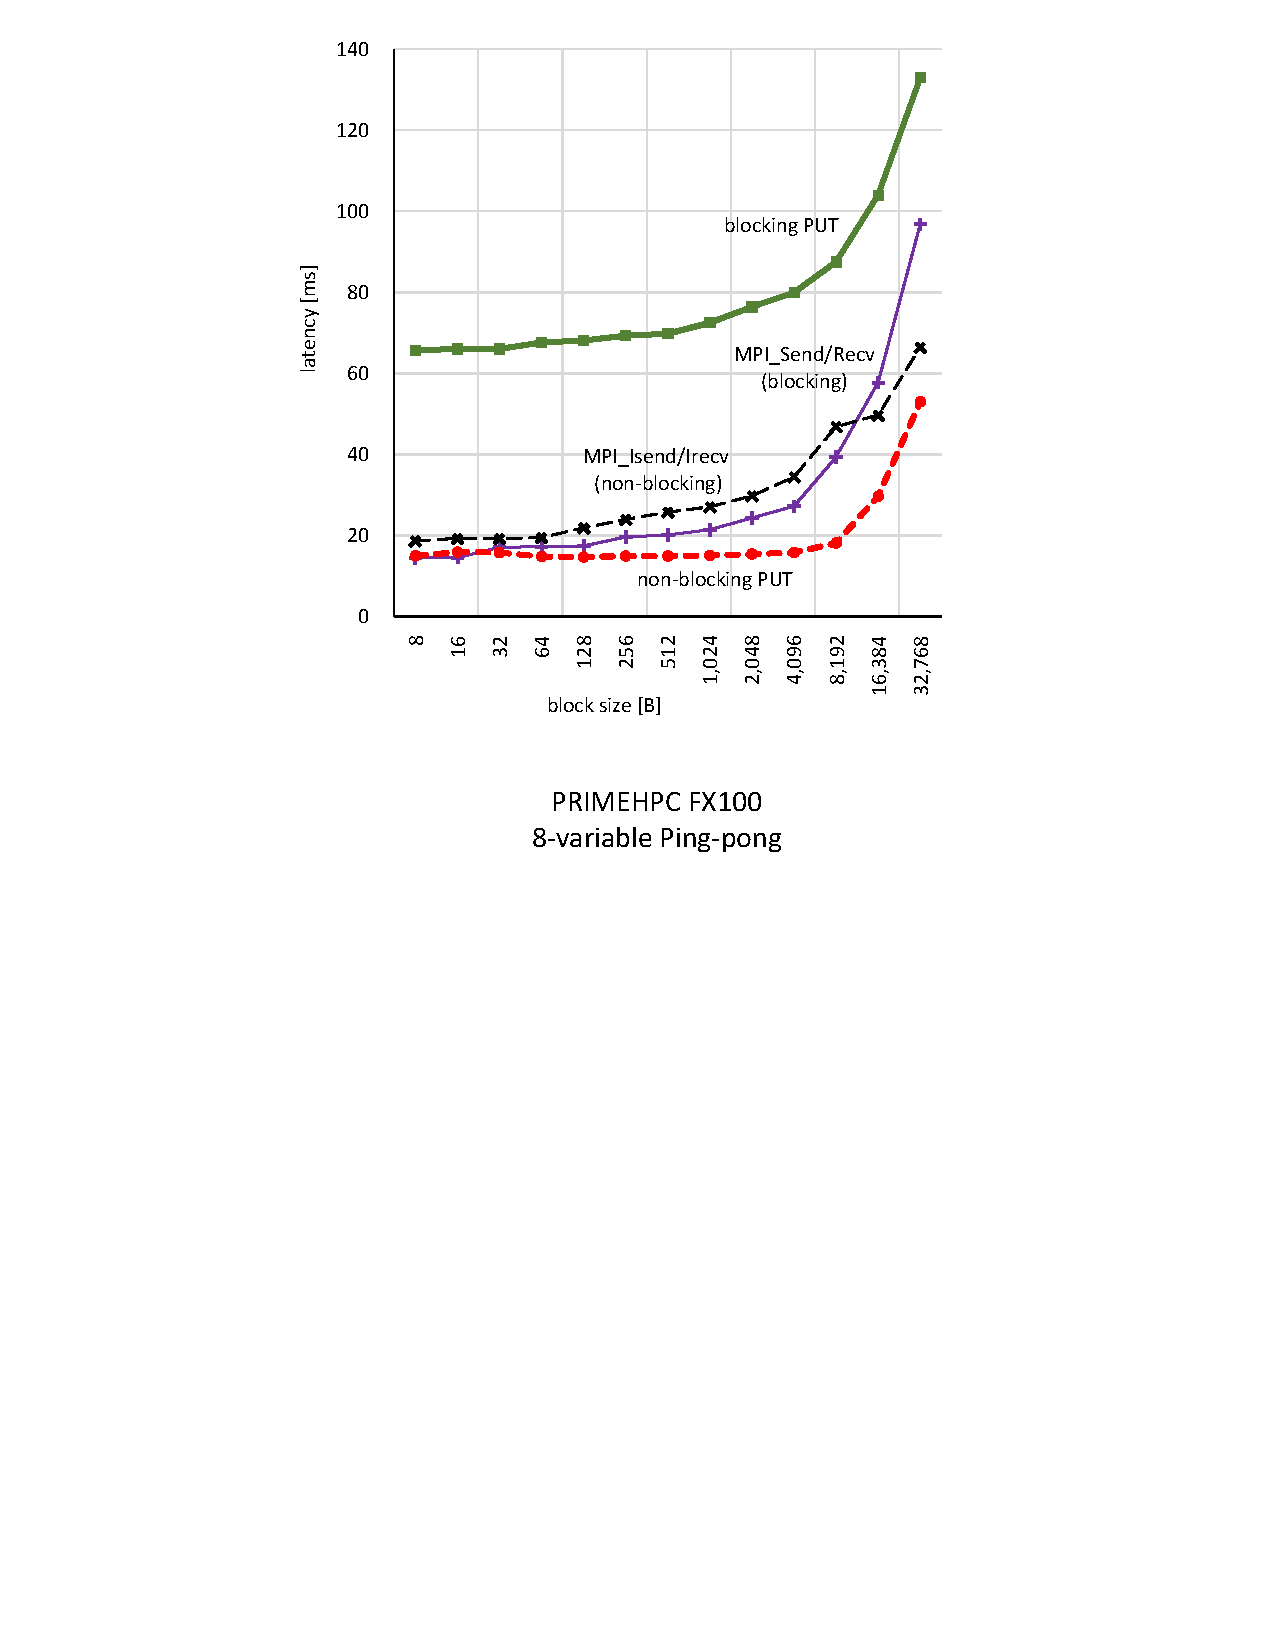
\includegraphics[trim=40mm 155mm 40mm 0mm, scale=0.6,clip]{figs/8var-pipo-latency.pdf}}\\
%    (b) Latency of blocking and non-blocking communications
%    \caption{8-variable ping-pong on PRIMEHPC FX100}\label{fig:8var-pingpong}
%   \end{center}
%\end{figure}



%===========================================================
\subsection{Himeno Benchmark}
%===========================================================


説明はどこかにある。\fig{himeno-graph}

%-- himeno-graph.pdf
\begin{figure}[p]
  \begin{center}
  % trimはleft bottom right topの順
    \mbox{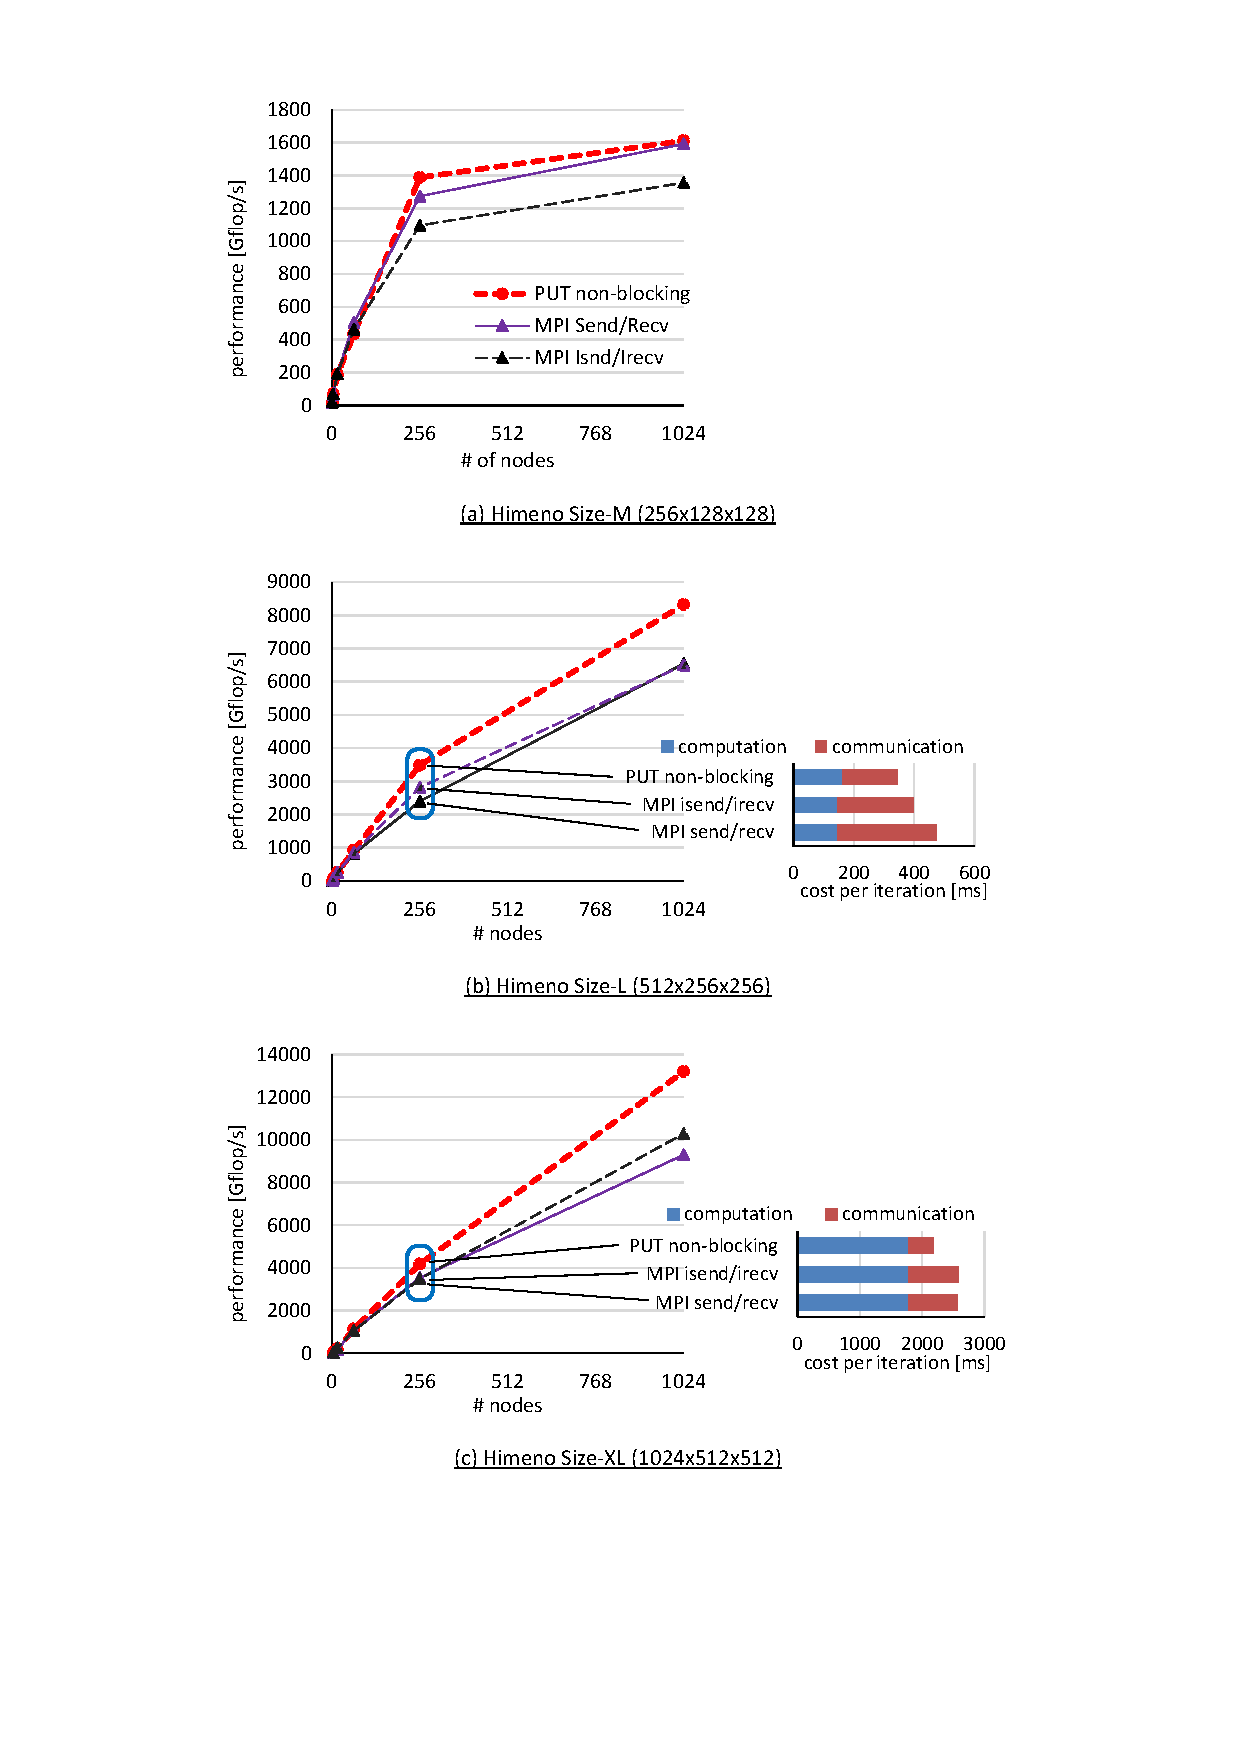
\includegraphics[trim=37mm 34mm 37mm 4mm, scale=0.8,clip]{figs/himeno-graph-r2.pdf}}
    \caption{himeno-graph-r2.pdf}\label{fig:himeno-graph}
  \end{center}
\end{figure}


マシン名要確認。ころころ変えていないか。


% %-- 3cell-y.pdf
% %-- 3cell-z.pdf
% \begin{figure}[tbh]
%   \begin{center}
%   % trimはleft bottom right topの順
%   \fbox{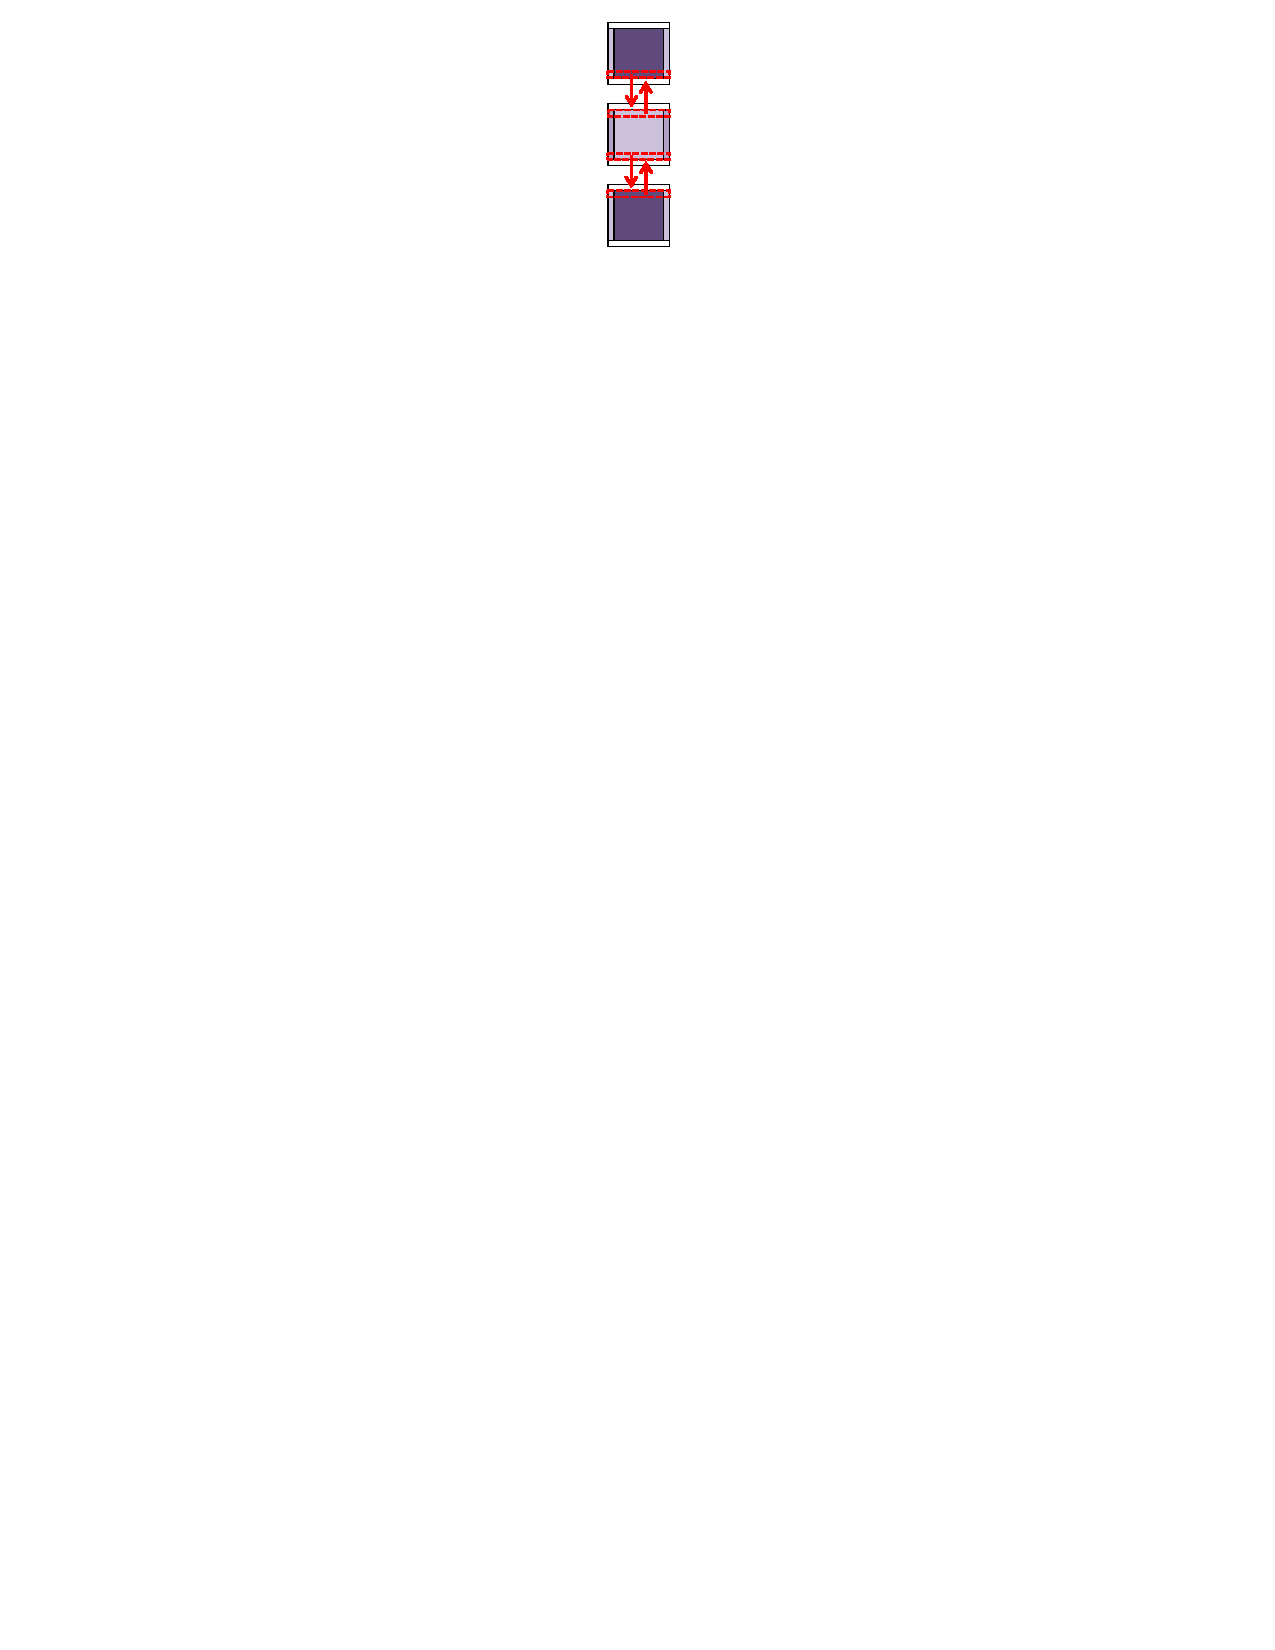
\includegraphics[trim=98mm 235mm 98mm 0mm, scale=0.8,clip]{figs/3cell-y.pdf}}  \\
%   \fbox{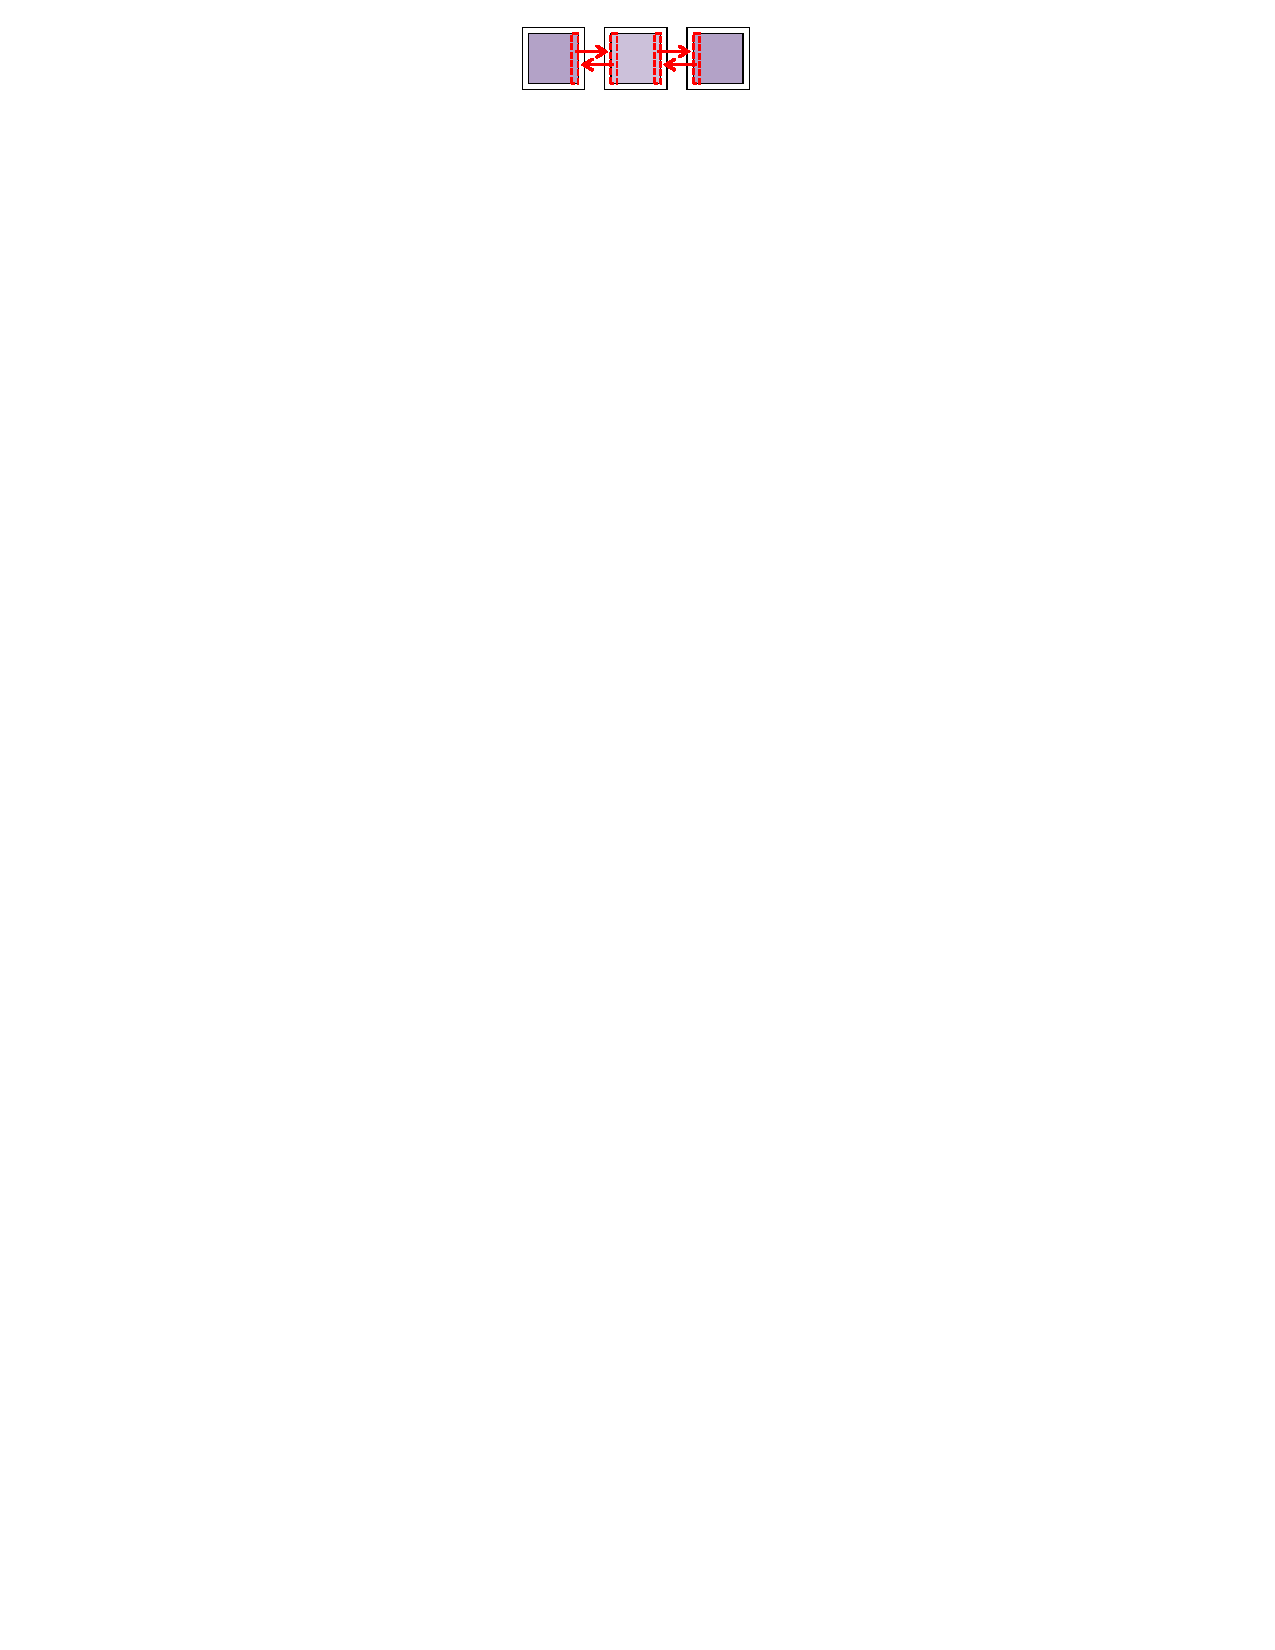
\includegraphics[trim=85mm 261mm 85mm 0mm, scale=0.8,clip]{figs/3cell-z.pdf}}  \\
%   \fbox{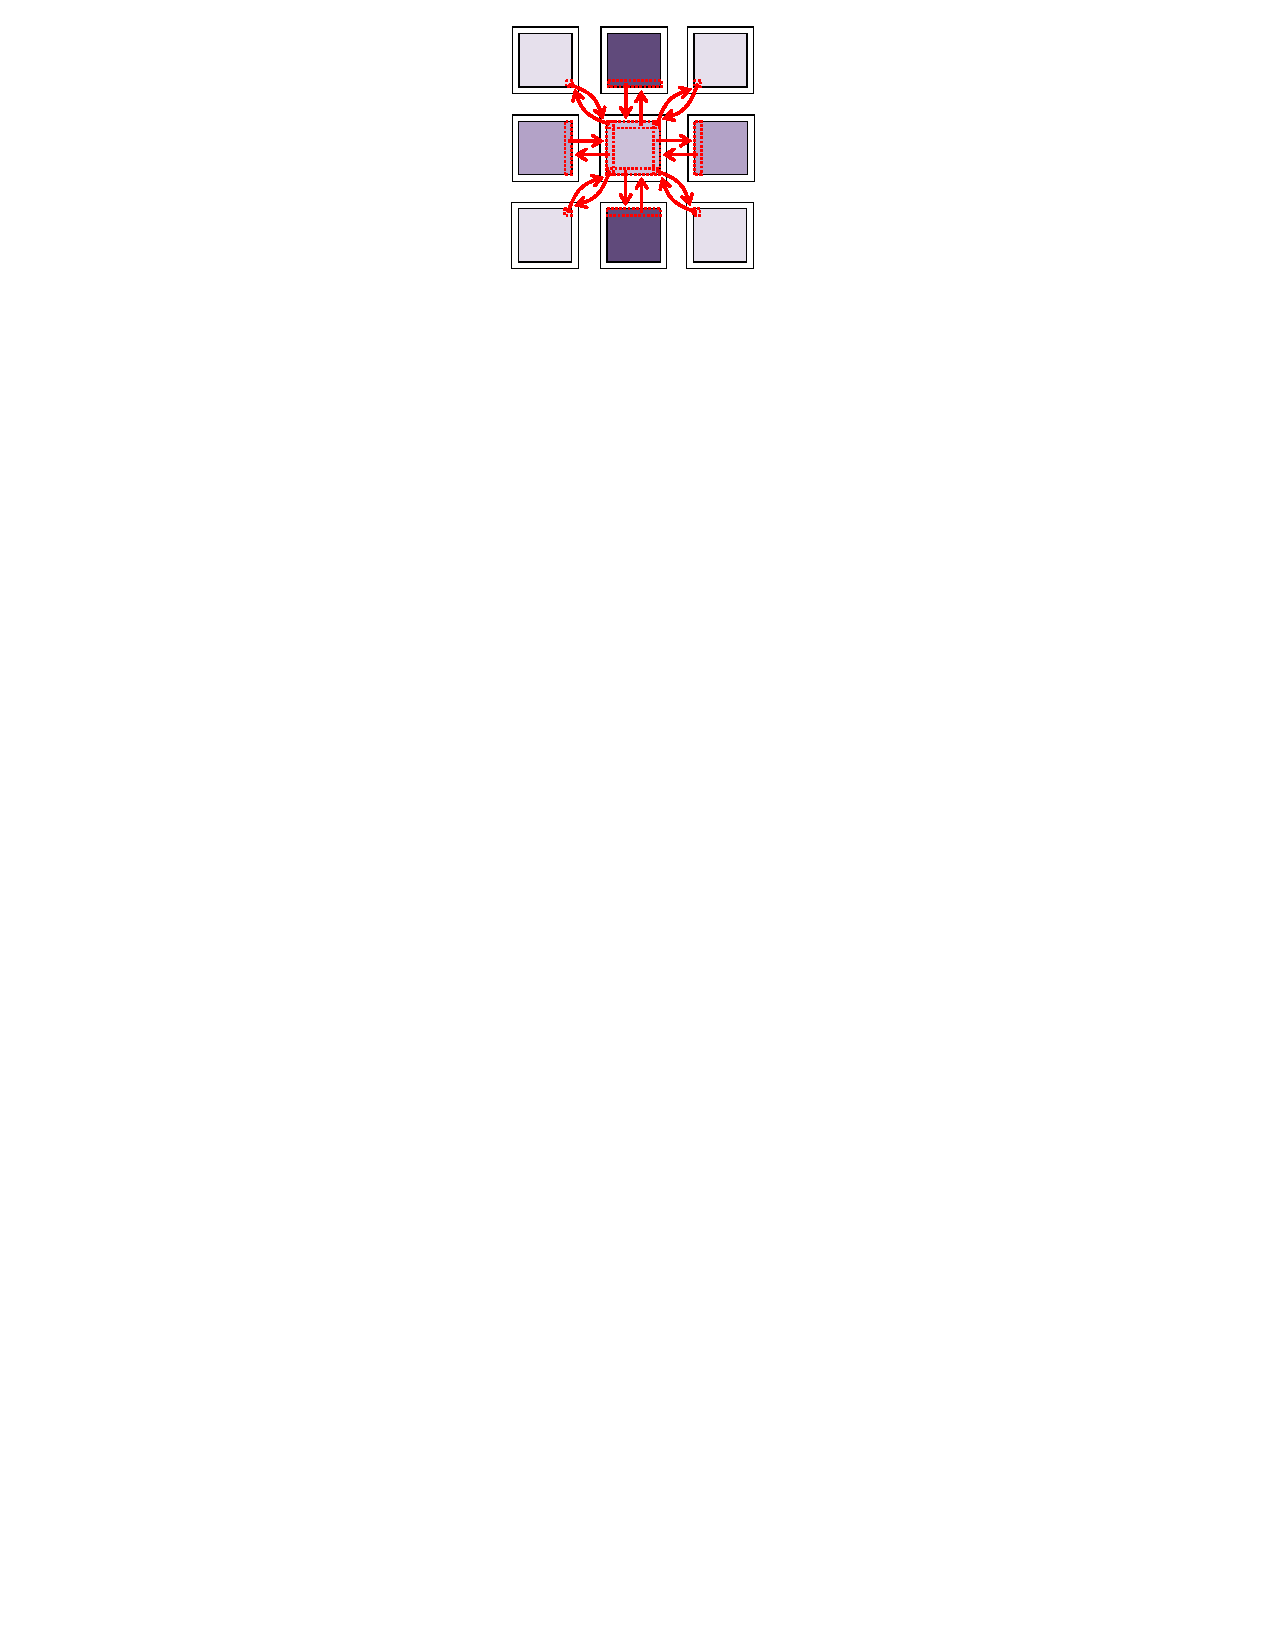
\includegraphics[trim=82mm 230mm 84mm 0mm, scale=0.8,clip]{figs/9cell-yz.pdf}}
%   \caption{3cell-y.pdf, 3cell-z.pdf, 9cell-yz.pdf}\label{fig:cell}
%   \end{center}
% \end{figure}


%-- fx100-pipo.pdf
%    \fbox{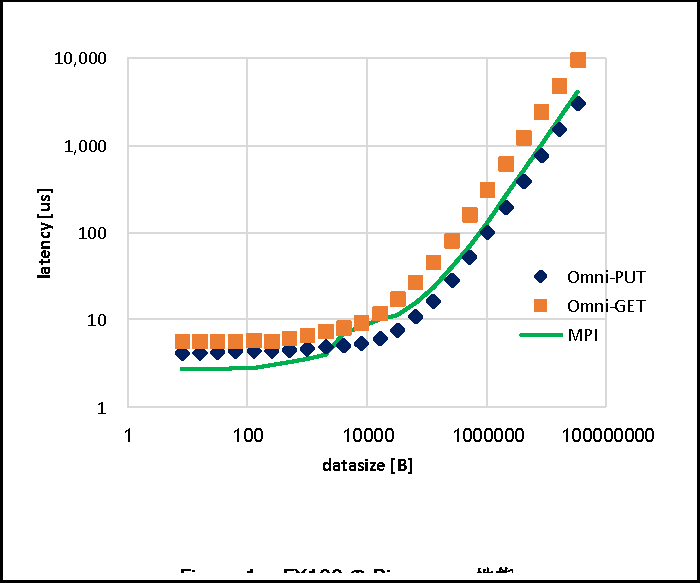
\includegraphics[trim=4mm 15mm 4mm 3mm, scale=0.9,clip]{figs/fx100-pipo.pdf}}

%himeno.pdf
%latency-16var.pdf
%layer.pdf

%register-CA-tmp.pdf
%register-RA-CA-tmp.pdf
%register-RA-tmp.pdf
%softstack.pdf
%translator-tmp.pdf

%\cleardoublepage

\section{Related Work}\label{sec:related}

%-- Coarray Imprementations
The University of Rice has implemented coarray features with their own extension 
called CAF2.0~\cite{Rice}.
It is a source-to-source compiler based on the ROSE compiler. GASNet is used as its 
communication layer.
Similarly to our RS and RA methods, they use the Cray pointer to pass the data 
allocated in C into Fortran.
%
Houston University developed UH-CAF onto the Open64-base OpenUH compiler~\cite{HU}. 
It supports coarray features defined in the Fortran 2008 standard. As the communication 
layer, GASNet and ARMCI can be used selectively.
%
OpenCoarrays is an open-source software project~\cite{OpenCo}. It is an library 
which can be used with GNU Fortran (gfortran) V5.1 or later. It supports coarray features
specified in Fortran 2008 and a part of Fortran 2018.  As the communication layer,
MPICH and GASNet can be used selectively.
%
In the vendors, Cray and Intel fully and Fujitsu partially support the coarray features
specified in Fortran 2008.

In the latest Fortran standard Fortran~2018, a subset of coarrays is called team.
It is similar to the executing images in the term of XMP, but does not affect
the parallel execution among images.

While non-blocking PUT communication is effective, non-blocking GET communication
is difficult to put into practical use because the acquired data is used immediately.
Cray has the directive extension for prefetching remote coarray corresponding to 
the GET communication.

Coarray C++ is a coarray implementation into C++. The coarray features are implemented
with the template library unlike XMP/C based on C language.


%\cleardoublepage

\section{Conclusion}\label{sec:concl}

This chapter described the coarray features in the context of XMP and 
the characteristic implementation of the coarray translator.

For memory allocation and registration, the RS, RA, and CA methods were
implemented corresponding to the communication library GASNet, FJ-RDMA,
and MPI-3.

For the coarray PUT and GET communications, DMA and four buffering methods
were described. The effect of the non-blocking PUT communication was
analyzed, and the knowledge is used to make the coarray version of the Himeno benchmark
from the original MPI version.
The measurement results on 1,024 nodes of the K computer, the coarray version 
is 27\% and 42\% faster than the original MPI version for Himeno sizes
L and XL, respectively.
The effect of the optimization of GET communication was also obvious on 
the ping-pong benchmark on HA-PACS/TCA and Fujitsu PRIMEHPC FX100.

As an evaluation of productivity, the coarray program uses fewer than half as
many characters as the MPI message passing program to write the same algorithm
as the Himeno benchmark.





%\cleardoublepage

\appendix

\section{MEMO}
%MPIはPGASに向かない、という論文がどこかに。

\section{Fusen}
\begin{verbatim}

synmetric memory
リモートのアドレスをローカルで計算できる
これがあるから、片側通信が。。。


下位層:通信libの差異を吸収し、上位層にプリミティブを提供する。
XMP coarray実装のプリミティブi/f
put operation
get operation
- どちらも連続データのみ/nonblocking。
sync memory operation
- 発行したputをすべてremoteに書き込み、getをすべてlocalに読み込むまで待つ。

putにはnonblocking技術:runtimeで十分
getにはprefetch技術:コンパイラ技術


生産性の観点の評価
1. リンク時にstatic配列を集めるところが対MPI片側通信で重要。言語仕様/言語処理系だからできる。単にライブラリ群/ライブラリ呼出しではできない。
2. F90配列記述がMPI_Typeの定義を不要にしている。


klogin7$ which xmpf90
~/Project/OMNI-clone/bin/xmpf90
klogin7$ xmpf90 --version
Version:1.3.1, Git Hash:4a5736e
klogin7$ 


sync memoryがいつ必要か
- ユーザ記述
- getのとき、1subarray参照に対してsyncmemoryを1回にする。
- getの前に、同じremoteアドレスへのputがあればsyncmemoryで待つ


alignmentの問題か
64バイト未満でputのlatencyが高い。
src5, RUN5で改善 ・・・しなかった
メモリ割付けのalignmentの問題ではない。
残るはTofuのputの単位の問題と推測
マスク付き書き込みになる?
この点ではRDMAよりバッファリングが有利


A Source-to-Source Translation of Coarray Fortran with MPI for High Performance
https://dl.acm.org/citation.cfm?id=3155888&dl=ACM&coll=DL

Preliminary Implementation of
Coarray Fortran Translator Based on Omni XcalableMP
https://ieeexplore.ieee.org/document/7306099

\end{verbatim}



\section*{Acknowledgments}
                                   
The present research used the computational resources of HA-PACS provided by the 
Interdisciplinary Computational Science Program at the Center for 
Computational Sciences at the University of Tsukuba. 

Part of the results is obtained by using the K computer at the RIKEN Advanced 
Institute for Computational Science (Proposal number ra000002). 




\begin{thebibliography}{99}
\addcontentsline{toc}{chapter}{\bibname}
 \bibitem{xmp} XcalableMP Language Specification, \url{http://xcalablemp.org/specification.html}
 \bibitem{mpi} MPI: A Message-Passing Interface Standard, \url{http://mpi-forum.org} (2015).
 \bibitem{coarray} John Reid, JKR Associates, UK. Coarrays in the next Fortran Standard.
    ISO/IEC JTC1/SC22/WG5 N1824, April 21, 2010.
 \bibitem{coarray18} ISO/IEC TS 18508:2015, Information technology -- Additional Parallel 
    Features in Fortran, Technical Specification, December 1, 2015.
 \bibitem{F08} Fortran~2008
 \bibitem{F18} Fortran~2018
 \bibitem{Rice} Rice University. Coarray Fortran 2.0. \url{http://caf.rice.edu/download.html}
 \bibitem{HU}
 \bibitem{OpenCo} OpenCoarrays \url{http://www.opencoarrays.org/}
 \bibitem{EPCC} EPCC Fortran Coarray micro-benchmark suite. 
    https://www.epcc.ed.ac.uk/research/computing/performance-characterisation-and-benchmarking/epcc-co-array-fortran-micro
 \bibitem{himeno} Himeno Benchmark. \url{http://accc.riken.jp/en/supercom/himenobmt/}

\end{thebibliography}


HPCAsia
\begin{verbatim}
[1]John Reid. 2010. Coarrays in the next Fortran Standard. ISO/IEC JTC1/SC22/WG5 
N1824, (Apr. 21, 2010)
[2]ISO/IEC 2015. Information technology – Additional Parallel Features in 
Fortran. ISO/IEC TS 18508:2015(E). (Dec. 2015)
[3]Rice University. Coarray Fortran 2.0. http://caf.rice.edu/download.html
[4]HPCTools Research Group at the University of Houston. OpenUH Open-source 
UH Compiler. http://web.cs.uh.edu/~openuh/
[5]OpenCoarrays. http://www.opencoarrays.org
[6]XcalableMP Specification Working Group. 2014. XcalableMP Language Specification 
Version 1.2.1. http://www.xcalablemp.org/specification.html
[7]Omni Compiler Project. http://omni-compiler.org
[8]Hidetoshi Iwashita, Masahiro Nakao, Mitsuhisa Sato. 2015. Preliminary Implementation 
of Coarray Fortran Translator Based on Omni XcalableMP. Proc. of 9th International 
Conference on PGAS Programming Models (PGAS2015), P.70-75, Washington, D.C. USA (Sep. 2015).
[9]Naoyuki Shida, Shinji Sumimoto, and Atsuya Uno. 2012. MPI Library and Low-Level 
Communication on the K computer, FUJITSU Scientific & Technical Journal, Vol.48, No.3, pp.324–330
[10]David Henty. 2012. A Parallel Benchmark Suite for Fortran Coarrays. In 
Applications, Tools and Techniques on the Road to Exascale Computing, Advances 
in Parallel Computing, Vol.22, pp.281-288.
[11]Himeno Benchmark. http://accc.riken.jp/en/supercom/himenobmt/
[12]Cristian Coarfa. 2007. Portable High Performance and Scalability of Global 
Address Space Languages. Ph.D. Thesis, Rice University (Jan. 2007).
[13]John Mellor-Crummey, Laksono Adhianto, William N. Scherer III, and Guohua 
Jin. 2009. PGAS ’09, Proc. of 3rd Conference on Partitioned Global Address 
Space Programming Models. Ashburn, VA, (Oct. 2009)
[14]Deepak Eachempati, Hyoung Joon Jun, and Barbara Chapman. 2010. An Open-Source 
Compiler and Runtime Implementation for Coarray Fortran. PGAS ’10, 4th Int’l 
Conf. on PGAS Programming Models, No.13.
[15]Shiyao Ge, Deepak Eachempati, Dounia Khaldi, and Barbara Chapman. 2015. 
An Evaluation of Anticipated Extensions for Fortran Coarrays, PGAS’15, 9th 
International Conference on Partitioned Global Address Space Programming Models, 
P47-58, Washington, D.C. USA (Sep. 2015).
[16]Alessandro Fanfarillo, Tobias Burnus, Valeria Cardellini, Salvatore Filippone, 
Dan Nagle, and Damian Rouson. 2014. OpenCoarrays: Open-source Transport Layers 
Supporting Coarray Fortran Compilers, PGAS ’14, Proc. of 8th International 
Conference on Partitioned Global Address Space Programming Models, No. 4.
\end{verbatim}

\end{document}



